\documentclass[12pt]{article}

% Encoding and font
\usepackage[utf8]{inputenc}
\usepackage[T1]{fontenc}
\usepackage{newtxtext,newtxmath} % Times-like font with math support

% Margins and layout
\usepackage[margin=1in]{geometry}

% Spacing
\usepackage{setspace}
\onehalfspacing
\setlength{\parindent}{1.5em}
\setlength{\parskip}{0pt} % No extra paragraph space
\usepackage{adjustbox}
% Figures and tables
\usepackage{graphicx}
\usepackage{subcaption}
\usepackage{booktabs}
\usepackage{tabularx}
% Footnotes
\usepackage{footmisc}
\setlength{\footnotesep}{0.5\baselineskip}

% Colors (optional, for emphasis/highlighting)
\usepackage{xcolor}
\usepackage{float}

% Bibliography: English, author-year style
\usepackage[style=authoryear,backend=biber]{biblatex}
\addbibresource{~/Sync/org-roam-mvm/bib/refs.bib}

% Title info
\title{The Form of Dissent: Measuring Preference Structure in Multiparty Contexts}


\author{}
%\author{Marcelo Veloso Maciel}
\date{} % Leave blank for no date

%The Form of Dissent: on the structuring of political polarization in Brazil
\begin{document}

\maketitle


\begin{abstract}
Polarization is usually measured by mapping citizens onto a one-dimensional ideological scale and summarizing the resulting distribution. This paper instead treats dissent as a property of ranked-preference profiles. In multiparty settings, citizens rank several alternatives, and political conflict may appear not only as ideological distance, but as organization in the space of rankings.

I develop a structure-sensitive measurement strategy that separates global reversal patterns, effective support, and group-level structuration. Globally, \(\Psi\), \(R\), \(HHI\), and \(RHHI\) distinguish pairwise antagonism, reversal mass, and reversal concentration. Effective-number diagnostics track whether dissent is diffuse across many rankings or compressed into fewer effective configurations. At the group level, \(C\) and \(D\) distinguish internal coherence from between-group divergence. I apply these diagnostics to ranked candidate preferences constructed from Brazilian CSES survey data from 2006, 2018, and 2022 using a nested resampling, imputation, and linearization pipeline.

The results show that Brazil's ranking profile becomes more conflictual and more organized between 2006 and 2022, but not as a collapse into two internally homogeneous camps. In 2006, dissent is present but relatively diffuse, with weak PT-centered structuration. In 2018, the profile becomes more conflictual and is organized most strongly by respondents' position toward Lula. By 2022, conflict is both higher and more compressed: pairwise antagonism and reversal mass rise, effective ranking and reversal-pair diversity fall, and ideology overtakes PT as the dominant structuring variable. The resulting pattern is compressed ideological structuration in a multiparty ranking space, not a simple binary division of the electorate. The results motivate a general point for comparative research: structure-aware metrics can register rising conflict without forcing electorates into binary representations, providing a portable template for dissent measurement in multiparty systems.
\end{abstract}


\textbf{Keywords:} political dissent; preference profiles; political polarization; multiparty systems; Brazil




\section{Introduction}

% Measures of political polarization often reduce disagreement to two opposing camps, overlooking the richer structure of preferences in multiparty settings. Using Brazilian Electoral Study data from 2006, 2018, and 2022, I analyze complete preference orderings over presidential candidates with two new metrics: RHHI that combines the proportion and concentration of opposed preferences, and G, a intragroup coherence and intergroup divergence measure. Results show that polarization between candidate pairs has intensified over time, but remains dispersed across multiple opposing preferences rather than concentrated in a single binary divide. By 2022, self-declared ideology emerges as the most salient source of preference structuring, overtaking traditional socio-demographic and partisan cleavages, including attitudes toward the Workers’ Party. The findings indicate that Brazilian political preferences are becoming more organized along ideological lines, yet retain a high degree of internal diversity, complicating prevailing narratives of a nation split into two antagonistic blocs.



% The discourse on polarization is shaped by two broad aspects: the near-universal intuition that polarization is both real and consequential, and the conceptual ambiguity surrounding what it actually is and implies. \textcolor{red}{mention the report}. Naturally, there are dissenters—some contest the idea that polarization is in fact occurring, while others question its relevance. Yet even this dissent is shaped by the same underlying ambiguity: the term “polarization” is overloaded, multidimensional, and depends on implicit theoretical commitments about why and how it matters. \textcolor{red}{summarize my contribution}





% - Intro
%   - global risk report for relevance
%   - implicit theoretical commitments, focus on binariness
%   - Brazil
%     - charactericstics that connect with my argument/contribution
% - My contribution


% the term “polarization” is overloaded, multidimensional,
% and depends on implicit theoretical commitments about why and how it matters.

% Political polarization is invoked as both an urgent democratic challenge and an empirical fact. Yet the concept itself is overloaded: it conflates distinct phenomena, is measured in incompatible ways, and often embeds hidden assumptions about why it matters. The prevailing empirical tradition treats polarization as either a widening gap in attitudes or an increased distance between ideal points in a latent space. These choices impose strong, often untested assumptions — shared response scales, single-peaked preferences — that are systematically violated in multiparty systems.

% Brazil offers a revealing test case. Its hyper-fragmented party system and coalition-driven presidentialism generate volatile alignments and shifting elite incentives, often read publicly as evidence of a ``deep divide.'' Nervertheless, most Brazilian polarization metrics still center on binary attitudes or coarse ideological self-placement, which are ill-suited to multiparty settings where voters simultaneously evaluate many alternatives. Moreover, comparative research on multiparty publics argues for \emph{group-sensitive} polarization measures (capturing both intergroup divergence and intragroup coherence) and while conceptual advancements \textcolor{red}{STUFF}  \parencite{bramson16_disam_social_polar_concep_measur}.


% Analyzing \emph{preferences over candidates}---complete or near-complete rankings---preserves ordinal structure and relational information that binary thermometers discard, aligning with recent advances that integrate voter preferences with party positions and that study ranking-based choice in real electorates \parencite{Hillen2019,Orriols2011}.


% This institutional backdrop helps explain why elite antagonism can spike even when mass left--right polarization is modest, a pattern consistent with broader multiparty findings that affective hostility can rise independently of ideological distance \parencite{Carlin2022,Gidron2020,Reiljan2020,Boxell2022}. In Brazil specifically, negative partisanship toward the PT (\emph{antipetismo}) structures voter identities and out-group animus, deepening affective divides even as programmatic sorting remains uneven \parencite{SamuelsZucco2018,Zucco2022}.



% This paper addresses that gap. Conceptually, it shows that the internal structure of preference profiles — not just first choices — contains crucial information about dissent that attitude- and ideal-point-based approaches miss. Methodologically, it applies for the first time the Can–Özkes–Storcken (2015) measure to empirical data and develops two new metrics: (i) RHHI, which combines the share of perfectly opposed rankings with their concentration; and (ii) G, which synthesizes intragroup coherence and intergroup divergence from estimated consensus rankings. Empirically, it applies these tools to Brazilian Electoral Study data for 2006, 2018, and 2022, revealing a shift toward more structured — yet still diffuse — fields of political preference, with self-identified ideology emerging in 2022 as the dominant axis of differentiation.

% The literature relies on at least two operationalizations of the attribute under analysis: attitudes and ideal points. This article proposes a shift in focus: from the analysis of  absolute evaluations (attitudes) to that of relative evaluations (preferences). Three contributions follow. (i) Conceptually, I demonstrate that the internal structure of preference profiles—not merely first choices—contains crucial information about dissent, while attitude-based and ideal-point approaches have their underlying assumptions violated. (ii) Methodologically, I am the first to apply the measure of \textcite{can2015measuring} to empirical data and introduce two complementary measures. The first, RHHI, captures the combination of the proportion of perfectly opposed rankings and their concentration; the second combines intragroup coherence and intergroup divergence with regard to their consensus rankings. (iii) Empirically, I apply these tools to simulations parameterized\footnote{This is a common design in the fields of social and public choice \parencite{kaminski2015empirical}.} by data from the \emph{Brazilian Electoral Study} (ESEB) for 2006, 2018, and 2022, showing that Brazil is undergoing a process of diffuse structuring and that, in 2022, self-identified ideology surpasses all other variables as the main axis of differentiation.






The global discourse on polarization is shaped by two  facets: the widespread intuition that political conflict is both real and consequential, and the persistent ambiguity surrounding what polarization actually is. Yet the concept remains overloaded. It is used to describe ideological distance, affective hostility, elite conflict, social sorting, partisan antagonism, and institutional deadlock. Even skeptical accounts, which question the extent or political relevance of polarization, often operate within the same conceptual ambiguity. The term carries implicit theoretical commitments about what kind of division matters, where it is located, and how it should be measured.

This ambiguity is especially consequential in multiparty settings. Much of the polarization literature relies on binary or one-dimensional representations, most commonly left versus right or government versus opposition. These representations are useful, but they foreground antagonism while often obscuring the organization of dissent itself. If citizens evaluate several alternatives, then political conflict is not exhausted by their location on a scale or by their first choice. It also appears in the structure of their relative evaluations: which alternatives are ranked together, which rankings are reversed, how concentrated those reversals are, and whether observable groups occupy distinct regions of the ranking space.

Brazil offers a useful vantage point for this problem. It is frequently described as deeply divided in journalistic and political discourse, and recent elections have been marked by intense elite conflict and affective antagonism \parencite{nunes2023biografia, samuels2018partisans}. At the same time, Brazil's multiparty presidential system, fragmented electoral field, and heterogeneous electorate make it difficult to assume that a single ideological axis captures the relevant structure of political disagreement. The empirical question is therefore not only whether Brazil is polarized, but how dissent is organized in the space of ranked candidate preferences.

 Dissent in multiparty electorates is not exhausted by attitudes, ideal points, or first choices. It also has a profile structure: a pattern in how citizens rank, reverse, cluster around, and separate among multiple alternatives. The contribution of the article is to develop diagnostics that make this structure observable and comparable. I develop diagnostics that describe how rankings are organized globally and across exogenous respondent partitions. Globally, \(\Psi\), \(R\), \(\kappa\), \(RHHI\), and effective-support summaries distinguish pairwise antagonism, reversal mass, reversal concentration, and the effective number of opposed rankings. At the group level, \(C\) and \(D\) distinguish internal coherence from between-group divergence.

I then apply these diagnostics to ranked candidate preferences constructed from Brazilian CSES survey data from 2006, 2018, and 2022. The application shows why the distinction matters. Dissent increases and the ranking space becomes more compressed, but the resulting structure is not reducible to a binary split. In 2018, Lula support is the strongest structuring partition; in 2022, ideology overtakes PT. The analysis therefore describes not only whether conflict rises, but what form that conflict takes in profile space. I also separate variability induced by resampling, imputation, and stochastic linearization to assess the robustness of these descriptive patterns.

The scope of the paper is descriptive and measurement-oriented. It provides a portable measurement strategy for comparative research on multiparty electorates, where conflict may increase without becoming binary, and where group structuration may occur without complete within-group consolidation. In \textcite{gerring12_mere_descr}'s terms, the core contribution is a set of indicators: measurement claims that map observed rankings to scales in order to describe specific dimensions of an object, while clarifying what later explanatory or causal analyses would need to account for. 

Section 2 reviews the literature on polarization measurement and argues that attitude-based and ideal-point approaches miss important features of ordinal preference structure. Section 3 defines the structure-sensitive diagnostics for ranked-preference profiles, including the global measures \(\Psi\), \(R\), \(\kappa\), \(RHHI\), effective-support summaries, and the group diagnostics \(C\) and \(D\). Section 4 describes the Brazilian CSES data, candidate-set construction, imputation, linearization, and uncertainty decomposition. Section 5 presents the empirical results for 2006, 2018, and 2022. The conclusion summarizes the argument and discusses how future work can extend these diagnostics to identify the candidate comparisons that generate internal dispersion or between-group divergence.



\section{Why Study Polarization in Preferences?}

The basic structure of the modal approach to polarization essentially consists of four elements: a set of agents, a set of attributes, a distribution over these attributes, and a measure defined on this distribution. Moreover, some notion of group, a partition of the set of agents,  is also assumed \parencite{bramson16_disam_social_polar_concep_measur, esteban1994measurement}.  Analyses of polarization usually focus on two groups, contrasting their evaluations of two attitude objects \parencite{fiorina08_polit_polar_americ_public, mason2015disrespectfully, iyengar12_affec_not_ideol}. Attitudes are absolute evaluative judgments directed at specific objects \parencite{holbrook2011attitude}. In political contexts, such objects are typically candidates, parties, organizations, or social groups. The set of agents is either citizens, or politicians. The main underlying group identifier tends to be political parties. However, recent work on mass polarization has sought to go beyond this binary framing  \parencite{kekkonen21_affec_blocs, rothers25_poles_polar, mehlhaff23_group_based_approac_to_measur_polar}, motivated by the fact that many countries exhibit an effective number of parties (ENP) greater than two. I propose by moving beyond the binary framework we should also extend the analysis to include relative evaluative judgments, that is, citizens' preferences. Why?



\begin{table}[h!]
  \centering
\begin{tabular}{lccc}
\toprule
\textbf{Person / Candidate} &  \textbf{C1} & \textbf{C2} & \textbf{C3} \\
\midrule
P1 & \textbf{100} & 60 & 0 \\
P2 & 60 & \textbf{85} & 70 \\
P3 & 50 & 55 & \textbf{60} \\
P4 & 52 & 56 & \textbf{60} \\
P5 & 51 & 54 & \textbf{59} \\
\midrule
Mean & 62.60 & 62.00 & 49.80 \\
\bottomrule
\end{tabular}
\caption{Feeling-thermometer scores. Bold indicates each respondent's most preferred candidate.}
\label{tab:mean}
\end{table}

First, attitude-based measures often summarize evaluations by averaging
responses across individuals \parencite{fuks22_polar_e_contex,
borba24_polar_ideol, mehlhaff23_group_based_approac_to_measur_polar}.
This operation is informationally demanding. Ranking candidates by average
thermometer scores does not only use each respondent's evaluation of the
alternatives; it treats score differences as commensurable across persons.
Formally, the comparison between two candidates \(a\) and \(b\) depends on
\(\bar{x}(a)-\bar{x}(b)
=
\frac{1}{n}\sum_i \bigl(x_i(a)-x_i(b)\bigr),
\) so a ten-point difference for one respondent is counted as the same
quantity as a ten-point difference for another. That is a substantive
interpersonal comparability assumption.

Table~\ref{tab:mean} illustrates the dependence of mean aggregation on this
assumption. The mean scores rank the candidates as \(C1 \succ C2 \succ C3\).
This ranking gives large aggregate weight to P1's use of the full
\(0\)--\(100\) range and combines it with the compressed \(50\)--\(60\)
ranges used by P3--P5. The calculation is mechanically valid, but its
interpretation requires more than the respondents' preference orderings: it
requires the numerical distances on their scales to be comparable across
persons.

By contrast, the ordinal information in the same table uses only each
respondent's internal ordering of the alternatives. It is invariant under
respondent-specific increasing transformations of the thermometer scale and
therefore does not require that a score of \(60\), or a difference of ten
points, have the same meaning across respondents. At the ordinal level,
three of the five respondents rank \(C3\) first, and pairwise majority
comparison produces \(C3 \succ C2 \succ C1\).\footnote{The point is not that
the ordinal ordering is the uniquely correct social ordering, or that
cardinal and ordinal summaries must coincide under full interpersonal
comparability. They need not. The point is one of informational
requirements: cardinal aggregation across persons presupposes interpersonal
comparability of score differences, whereas ordinal profiles require only
within-person comparisons.} For this reason, preference profiles provide a
more conservative informational basis for studying polarization when
interpersonal comparability of thermometer scores is not independently
secured \parencite{narens2007introduction}.


% Second, because even though analyses based on ideal points—\emph{i.e.}, on models that locate voters and alternatives in a space and define utility as a (typically) decreasing function of distance—would, in principle, characterize a preference-based study, they start from a spatial representation that presupposes single-peaked preferences \parencite{elkind2022preference, fiorina08_polit_polar_americ_public}, an assumption routinely violated in large-scale survey data \parencite{regenwetter2006behavioral, feld1988ideological}. A unidimensional Euclidean representation of preferences implies single-peakedness; therefore, by contraposition\footnote{This follows from basic classical logic \parencite{da2008ensaio, velleman2019prove}. For any formulas $A, B$, we have $(A \to B) \leftrightarrow (\neg B \to \neg A)$.}, the failure of single-peakedness implies the impossibility of such a representation. More concretely: the spatial model embeds alternatives in an outcome space and assigns each voter a most-preferred point (a “bliss point”); all alternatives are ranked by their distance from that point. This construction \emph{requires} that each voter’s preference be single-peaked along the relevant ordering, so that utility falls as one moves away from \textit{the} peak. If a voter’s preference is not single-peaked—\emph{e.g.}, it has two local maxima—then no single point can summarize that voter’s tastes, and distance from the  “ideal point” will fail to recover the observed ranking (moving away from the designated peak can increase, rather than decrease, utility). Consequently, if there is no ordering of the alternatives under which \emph{all} voters’ preferences are single-peaked, a one-dimensional Euclidean (ideal-point) representation is misspecified: distances from putative ideal points will not preserve individual orderings, and aggregation based on those points/distances inherits this mismatch. In survey data, this violation for citizens’ rankings over candidates is not difficult to demonstrate and has been known for decades \parencite{ballester10_charac_singl_peaked_domain, feld1988ideological}. The problem does not arise in bipartisan contexts, as these are vacuously single-peaked\footnote{A vacuously true proposition is a statement considered true because there are no objects satisfying the conditions of the antecedent. In the case of the single-peakedness of a profile with only two alternatives, there are only two possible ways to order these alternatives, and in both all preferences will have a unique peak. Equivalently, there is a characterization of the single-peakedness of a profile in terms of forbidden subprofiles: a criterion with 3 agents and 3 alternatives, and another with 2 agents and 4 alternatives \parencite{ballester10_charac_singl_peaked_domain}. Now, with only 2 alternatives, it is impossible to violate these criteria.}.



Second, while unidimensional Euclidean ideal-point methods are preference-based, they rely on a spatial representation that presuppose single-peakedness on the  profile \parencite{elkind2022preference}. Spatial models locate voters and alternatives on a line and define utility as decreasing in distance from each voter's ideal point. This construction implies that, along the relevant ordering of alternatives, each voter has a single peak and ranks alternatives lower as they move farther from that peak. Hence, if no ordering of the alternatives makes the observed profile single-peaked, a unidimensional Euclidean representation cannot preserve the individual rankings.\footnote{This claim concerns unidimensional Euclidean representations. Single-peakedness is not a necessary condition for embeddings in higher-dimensional spaces.}

This is not a marginal concern. Violations of single-peakedness in citizens' rankings over candidates is widespread on survey data \parencite{regenwetter2006behavioral, feld1988ideological, ballester10_charac_singl_peaked_domain}. In such cases, distances from putative ideal points do not recover the ordinal information contained in voters' preferences, and aggregation based on those points inherits the mismatch. The problem is muted in two-alternative settings, where single-peakedness is vacuous, but it becomes substantive as soon as voters rank three or more alternatives. This is precisely the setting in which multiparty electorates require methods that preserve more of the structure of preference profiles.

\begin{table}[htbp]
\centering
\caption{Preference profiles with the same first choices but differing structure}
\label{tab:profile-matrix}
\begin{tabular}{ll}
\toprule
\textbf{Profile 1} & \textbf{Profile 2} \\
\midrule
ABCD & ADCB \\
ABDC & ADCB \\
ACBD & ADCB \\
ACDB & ADCB \\
ADCB & ADCB \\
ADBC & ADCB \\
BACD & BCDA \\
BADC & BCDA \\
BCAD & BCDA \\
BCDA & BCDA \\
BDAC & BCDA \\
BDCA & BCDA \\
\bottomrule
\end{tabular}
\end{table}


Third, when there are more than two alternatives, important patterns, such as partial agreements or localized dissent, tend to be obscured. The resulting narrative becomes reductive and potentially misleading. Consider the preference profiles presented in Table~\ref{tab:profile-matrix}. Each row represents the preference of a voter. For example, in row 1 of Profile 1, the voter strictly prefers A over B over C over D. If we assess polarization solely on the basis of voters’ first choices, these two profiles appear identical and equally polarized. However, this interpretation does not withstand closer scrutiny, due to the substantial loss of information involved in reducing polarization to the distribution of first preferences. Such an approach completely ignores the underlying structure of support for alternatives C and D. Profile 1 exemplifies maximal diversity beyond the first choices, A and B. Every possible ranking involving the alternatives B, C, D and C, A, D occurs with equal probability in the subprofiles. That is, if we split Profile 1 into groups based on first choices, with one group preferring A and the other preferring B, we observe minimal internal coherence within each group.

Profile 2, by contrast, reveals a distinct structure. When divided by first choices, it displays maximal internal coherence, since each group is internally unanimous, and maximal intergroup divergence, because the rankings of voters who prefer A are completely reversed relative to those who prefer B. Remarkably, however, Profile 2 also reveals a consensus absent in Profile 1. The alternatives C and D appear more inclusive than A and B \parencite{igersheim22_compar_votin_method}. The visible “polarization” therefore conceals an underlying consensus, as C and D are broadly acceptable.

This analytical example gains relevance when contrasted with narratives based on margins of victory. Consider the 2022 Brazilian presidential election, which \textcite{nunes2023biografia} cites as blatant evidence of a deeply polarized country. Lula won the second round, under a majority-with-runoff system, with 50.9\% of valid votes, compared to 49.1\% for Bolsonaro, a margin of less than one percentage point. This was the closest victory in the history of Brazilian presidential elections. The second closest occurred in 2014, when Dilma won with 51.64\% against 48.36\% for Aécio Neves. Does this imply that the country was polarized? As the analytical example shows, any conclusion must be qualified by the rest of citizens’ rankings.

Accordingly, there is a need for alternative measures that more faithfully capture the structure of preference profiles. Even within attitude-based approaches, polarization is a multidimensional concept \parencite{bramson2017understanding, bramson16_disam_social_polar_concep_measur}. It is therefore unlikely that any single measure can adequately capture it \parencite{patty14_analy_big_data}.


\section{Global and Group Structure in Preference Profiles.}

We now turn to the development of measures that can capture the internal structure of preference profiles. The challenge lies in designing indices that are sensitive not only to the distribution of first choices, the traditional focus of polarization research,but also to the patterns of agreement and disagreement that emerge across the full ranking of alternatives.

\textcite{can2015measuring} propose a measure of polarization that can be applied to profiles of linear orders\footnote{A \emph{strict linear order} on a non-empty set \(X\) is a binary relation \(<\) that is (i) {irreflexive}: \(\lnot(x<x)\) for all \(x\in X\); (ii) {transitive}: \(x<y\land y<z\!\implies\! x<z\); and (iii) {trichotomous}: for any distinct \(x,y\in X\), exactly one of \(x<y\) or \(y<x\) holds.  }, but it has not yet been empirically mobilized. Let \( \mathcal{L} \) be the set of linear orders on a finite set of alternatives \( A \). Given a profile \( p \in \mathcal{L}^N \) two distinct alternatives \( a, b \in A \), we define \( n_{ab}(p) = \# \{ i \in N : (a, b) \in p(i) \} \), the number of individuals who prefer \( a \) over \( b \); and  \( d_{ab}(p) = |n_{ab}(p) - n_{ba}(p)| \), the absolute difference in relative support between \( a \succ b \) and \( b \succ a \) in the population. If \( n \) is the number of agents,  \( m \) is the number of alternatives, and \(\bar{A}\) is the set of all subsets of \(A\) of size 2,  then the measure is given by:

\[
\Psi(p) = \sum_{\{a,b\} \in \bar{A}} \frac{n - d_{ab}(p)}{n \cdot \binom{m}{2}},
\]


Despite its elegance, the measure \(\Psi\) has relevant limitations. It considers
only global margins between pairs of alternatives—that is, the aggregate
disagreement between pairs. It is not really using the preference information. Note that \(\Psi\) is just a summation of margins of victories, normalized by  the number of pairs of alternatives. We could have a list of incomplete pairwise evaluative judgements (\(x\succ_{i}y\), for not all alternatives), or even voters with cyclic preferences  and the measure would be insensitive to these variations. As such, it  completely ignores structural features of
profiles, such as the formation of clusters of preferences
\parencite{bramson16_disam_social_polar_concep_measur}. This insentivity to the structure of the profiles implies that disparate profiles with the same margins of victory will be considered equally polarized. To present an extreme and relevant case first let's note that the reversal of an ordering \( abcd \) is \( dcba \). Now,
note that \(\Psi\) assigns the maximum value \(1\) both to: a uniform profile, in
which all possible linear orders are equally probable (with probability \(1 \over {m!}\)), and to a profile
composed of any two reversed preference orders with equal proportion of \(1 \over 2\).

% \(\{ r_1 : \tfrac{1}{m!}, \ldots, r_{m!} : \tfrac{1}{m!} \}\)

% : \(\{ r_\star : \tfrac{1}{2},\ -r_\star : \tfrac{1}{2} \}\)

One can remain agnostic as to which of the two profiles should be regarded as
``more polarized.'' Analogous to what is argued in Section~2, the first profile
exhibits maximal diversity, whereas the second is highly concentrated on a
single opposition. In the latter, however, certain candidates remain
relatively consensual, eliciting neither strong rejection nor strong approval.
It is  desirable to differentiate between these configurations, though, and
\(\Psi\) fails to do so.

Moreover, recent literature has increasingly emphasized the explicitly
group-based nature of the concept of polarization
\parencite{mehlhaff23_group_based_approac_to_measur_polar,
  bramson2017understanding}. Conceptually, a influential formulation of
polarization\footnote{\textcite{bramson2017understanding, bramson16_disam_social_polar_concep_measur}
identify nine distinct senses of polarization; the specific combination of
these senses adopted yields different conceptualizations, and hence different
measures, of polarization.} treats it as the joint occurrence of high
intragroup coherence and high intergroup divergence. The measure \(\Psi\),
however, is defined globally for the entire profile and does not incorporate a
group structure. It therefore cannot serve as an operationalization of
polarization under this group-based conception.


The first step to distinguish between preference profiles is to actually operate
with the rankings rather than with the aggregated pairwise comparisons. Note
that a natural idea of polarized preferences is the opposition between rankings
and their reversals. From a micro perspective, reversed preferences are those
that exhibit the maximum distance according to standard metrics
\parencite{zwicker2016introduction};
they therefore represent the case of maximum disagreement between two agents.
Note also that, from a macro perspective, the more reversed preferences we add
to a profile, the more we inflate the value of \(\Psi\). The fraction of the
profile composed of directly opposing orderings capture features of the profile
that foster global disagreement and are guaranteed to increase \(\Psi\). To
calculate this fraction first define the degree of opposition, or balance,
between an ordering \( r_i \) and its reversal \( -r_i \) as:
\[
\text{op}(r_i) = 2 \cdot \min(p(r_i), p(-r_i)),
\]
where \( p \) denotes the proportion of each ordering in the profile. The total opposition in the profile is then given by:
\[
R = \sum \text{op}(r_i),
\]
summing over the unique orderings \( r_i \), so as to avoid double counting of reversed pairs.

To incorporate the notion of concentration, the Herfindahl–Hirschman Index (HHI) is applied to the proportions of reversal. Thus, define \( q_{i} = {\text{op}(r_i) \over R} \), and we have
\[
\kappa = \sum_{i} q_{i}^{2}.
\]
The final measure, \( \mathrm{RHHI} \), is defined as the geometric mean between the degree of opposition and its concentration:
\[
\mathrm{RHHI} = \sqrt{R \times \mathrm{kappa}}.
\]

Why a product, rather than, say, an arithmetic mean? Because the construct we
want is explicitly \emph{conjunctive}: it should be large only when two features
co-occur, namely (i) a substantial mass of perfectly opposed preference pairs
($R$) and (ii) a strong concentration of that opposition around a small set of
pairings ($\kappa$). Either ingredient on its own describes a different situation:
high $R$ with low $\kappa$ is widespread but diffuse antagonism, while low $R$ with
high $\kappa$ is concentrated but small-scale antagonism. An arithmetic mean would
treat these components as partially interchangeable by allowing one to
compensate for the other, thereby assigning high scores to profiles that lack
one of the defining ingredients. The geometric mean enforces the intended ``both
at once'' logic: it increases only when both inputs increase, collapses toward
zero when either component is near zero, and penalizes imbalance while remaining
symmetric in $R$ and $\kappa$. An interesting measure that can be derived from \(\kappa\) is the  \emph{effective number of pairs of reversed preferences} (ENRP), by analogy with the effective number of parties \parencite{shugart2017votes} and is defined as \(ENRP = 1/\kappa\), which facilitates the interpretation of values of \(\kappa\). Given this connection between \(RHHI\) and the dispersion of the profile, I also consider the \emph{effective number of observed rankings} (EO) as a diagnostic in the analysis.


% \footnote{Another possibility would be to apply maximum likelihood estimation (MLE) of mixtures of Mallows models over a sequence of integers to identify clusters of voters, penalizing for model complexity using an information criterion \parencite{mcelreath2020statistical}, in order to determine the optimal number of groups and their associated consensus rankings. The problem is that there are no packages that do this directly for preference data.}


The simplest way to implement a group-based measure of profile structuration, while preserving the full information of orderings, is to evaluate exogenous groupings such as race, sex, religion, ideology, or candidate support. For each group, I estimate a consensus ranking directly from the observed rankings rather than assuming a parametric ranking model. Let \(\mathcal{L}(A)\) be the set of all linear orders over the active candidate set \(A\). For a group \(g\), with members \(i \in g\) and observed rankings \(\rho_i \in \mathcal{L}(A)\), define the total Kendall loss of a candidate consensus ranking \(\rho \in \mathcal{L}(A)\) as
\[
L_g(\rho) = \sum_{i \in g} d_{\tau}(\rho_i,\rho),
\]
where \(d_{\tau}\) is Kendall tau distance. The group consensus set is then
\[
M_g = \arg\min_{\rho \in \mathcal{L}(A)} L_g(\rho).
\]
Thus, the consensus is  a ranking, or set of rankings, that minimizes the total distance to the group's observed preferences.

When \(M_g\) contains more than one ranking, I do not impose an arbitrary tie-breaking rule. Instead, group-level quantities that depend on the group consensus are averaged over all minimizing rankings in \(M_g\). This preserves the ambiguity generated by the profile itself. Once the consensus set of each group is obtained, it becomes possible to measure intragroup coherence and intergroup divergence.

We start with the coherence of a group \(g\), defined in terms of the average Kendall tau distance between the group members' rankings and the group's consensus set. The Kendall distance, \(d_{\tau}\), quantifies the disagreement between two orderings by counting the number of pairs of alternatives ordered differently \parencite{zwicker2016introduction}. For a group \(g\) of size \(n_g\), the consensus-relative average distance is:

\[
\text{AvgDist}_g = \frac{1}{n_g}\sum_{x \in g} \frac{d_{\tau}(x, \rho_g)}{\binom{m}{2}}.
\]
The coherence of group \( g \) is then defined as:
\[
C_g^{\star} = 1 - \text{AvgDist}_g.
\]
Thus, \( C_g^{\star} = 1 \) if all members share exactly the ordering \( \rho_g \), and it decreases as internal divergence increases. We aggregate these coherences into a global score weighted by group size:
\[
C^{\star} = \frac{1}{n} \sum_{g=1}^{k} n_g\,C_g^{\star}, \quad\text{with } n = \sum_{g=1}^{k} n_g.
\]
A key correction is that \(C^{\star}\) is not bounded below by \(0\), but by \(1/2\). Intuitively, because \(\rho_g\) is chosen to minimize average Kendall distance, for each pair of alternatives one can orient \(\rho_g\) to agree with at least half of the group on that pair; hence the fraction of pairwise disagreements cannot exceed \(1/2\), so \(\text{AvgDist}_g \le 1/2\) and therefore \(C_g^{\star} \ge 1/2\) (and likewise \(C^{\star} \ge 1/2\)).

Since \(1/2\) functions as a natural ``no-structure'' baseline, we rescale coherence to place this baseline at zero:
\[
C \;=\; 2C^{\star}-1,
\]
so that \(C \in [0,1]\), with \(C=0\) corresponding to coherence no better than the baseline and \(C=1\) corresponding to perfect within-group unanimity.


Let \( k \) be the number of identified groups and \( n_i \) the size of group \( G_i \). Let \( \rho_j \) denote the consensus ordering of group \( j \). We define the measure of divergence between groups \( D \) as:
\[
D = \frac{1}{(k-1)} \sum_{i \neq j} \frac{n_i}{n} \cdot \left(\frac{1}{n_i}\sum_{x \in G_i} \frac{d_{\tau}(x, \rho_j)}{\binom{m}{2}}\right).
\]


The expression can be understood as follows. The sum \(\sum_{i \neq j}\) runs
through all ordered pairs of distinct groups, so we divide by \((k-1)\) to
ensure normalization. Each group is weighted by its relative size using the
factor \( n_i / n \). The distance term \( d_{\tau}(x, \rho_j) \) represents how
far an individual in group \( G_i \) is, on average, from the consensus ordering
of another group \( G_j \), normalized by the total number of pairwise
comparisons. Finally, the inner mean,
\( \frac{1}{n_i}\sum_{x \in G_i}(\cdots) \), captures this average distance
across all members of \( G_i \) relative to the consensus ordering of \( G_j \).
The value of \( D \) increases as the groups become more distinct from each
other and equals zero if all preferences are essentially identical.


The measure \(D\) captures how far the members of one group are from the consensus rankings of other groups. For this reason, it is useful as a measure of external divergence, but it is not a pure between-group statistic. If a group is internally dispersed, its members will already be far from their own consensus, and this dispersion carries over into their distances to other groups' consensuses. Thus, a high value of \(D\) can reflect either genuine distance between group consensuses or the fact that the group is internally spread out. This is why I keep \(C\) and \(D\) separate. The raw coherence \(C^{\star}\) implies a within-group dispersion term \(1-C^{\star}\), and Appendix~\ref{app:c-d-relationship} shows that
\[
D \geq 1-C^{\star} = \frac{1-C}{2}.
\]
Combining \(C\) and \(D\) into one scalar would therefore hide whether a partition structures the ranking profile through internal coherence, external divergence, or both.

For this reason, I do not combine the group diagnostics into a single polarization score. A composite measure would obscure the distinction between internal coherence and external divergence. Instead, I treat \(C\) and \(D\) as a diagnostic pair. The goal is not to assign each partition one scalar value of polarization, but to describe how, and in what sense, an exogenous grouping structures the preference profile. In this sense, the paper extends the disambiguation strategy of \textcite{bramson2017understanding, bramson16_disam_social_polar_concep_measur} from one-dimensional attitude distributions to ranked-preference profiles: rather than asking whether an electorate is polarized in general, the analysis asks which structural features of dissent are present, and how they vary across time and partitions.

The diagnostics can be read against three benchmark profiles: unanimity,
equiprobability, and pure inversion. In a unanimous profile, all respondents
hold the same ranking. There is no pairwise antagonism, no exact reversal mass,
and no reversal concentration to measure. In a pure inversion profile, by
contrast, half the respondents hold a ranking and half hold its reversal. Every
pairwise comparison is then evenly split, all profile mass lies on one opposed
ranking pair, and opposition is maximally concentrated. This is the limiting
case of organized antagonism in the ranking space.

The equiprobable profile gives the contrasting case. If all rankings occur with
equal frequency, every pairwise comparison is also evenly split, so pairwise
antagonism is maximal. Exact reversal mass is maximal as well, because every
ranking is matched by its reversal. But the structure is not the same as in the
pure inversion profile: reversal mass is dispersed across all possible reversal
fields rather than concentrated in one of them. This is why \(\Psi\) and \(R\)
must be distinguished from \(\kappa\), \(RHHI\), and \(ENRP\). The former
identify the amount of pairwise or exact opposition in the profile; the latter
identify whether that opposition is concentrated in a small number of reversal
fields or diffused across many ranking configurations. An analogous logic
applies to the group measures. Appendix~\ref{app:measures-action} reports the
formal behavior of the measures on these reference profiles.






\section{Empirical Evidence from Brazil (ESEB 2006–2018–2022)}
% We now turn to the empirical application. I use data from the ESEB for the years 2006, 2018, and 2022. Brazil, as a multiparty system, is frequently cited as an exemplary case of political polarization\parencite{nunes2023biografia, borba24_polar_ideol}. These years were chosen to allow for a comparison between a period of low polarization (2006), at least intuitively, and periods of pronounced polarization (2018 and 2022).



We now turn to the empirical application, drawing on data from the Estudo Eleitoral Brasileiro (ESEB) - which is associated with the Comparative Study of Electoral Systems for the years 2006 (n = 1000), 2018 (n = 2506), and 2022 (n = 2001). Brazil’s multiparty presidential system has been invoked as a paradigmatic case of  polarization, with its combination high electoral fragmentation, weak programmatic structuring, and the salience of a single polarizing party, the Workers’ Party (PT), as a stable focal point of partisan affect \parencite{samuels2018partisans, nunes2023biografia}. The selected years correspond to qualitatively different political contexts as described in existing accounts of Brazilian competition and alignment.

The 2006 election took place during a period generally interpreted as one of relatively low mass polarization, despite growing elite antagonism following the mensalão corruption scandal. This contrasts sharply with 2018, widely recognized as a watershed moment of intense partisan and ideological polarization, marked by Jair Bolsonaro’s rise and the consolidation of a strongly anti-PT bloc \parencite{samuels23_partis_stereot_polar_brazil}. The 2022 contest supposedly further entrenched this bipolar dynamic, producing the most competitive and contentious presidential race since redemocratization, with polarization manifesting both in elite rhetoric and in voter behavior \parencite{nunes2023biografia}. Comparing these three waves allows a descriptive assessment of how preference-profile structure differs across periods commonly discussed in polarization narratives.

The analysis is based mainly on the ESEB feeling-thermometer question, which asks
respondents to rate political leaders on a scale from \(0\) to \(10\), where
\(0\) means that the respondent does not like the figure at all and \(10\)
means that they like the figure a lot. Responses indicating that the respondent
does not know the politician, does not know how to answer, or did not answer
are treated as missing values.

This question is a thermometer scale and can therefore be interpreted as a weak
order\parencite{regenwetter2006behavioral}\footnote{A complete, reflexive, and transitive relation.}. The list of political figures includes both declared
presidential candidates and individuals publicly floated as potential contenders
for the office. Although there are minor coding variations between the datasets for the three years, the procedure is analogous.





The starting point for the analysis is the construction of weighted
pseudo-profiles, following the resampling strategy proposed by
\textcite{popov2014consensus} and used in empirical social choice applications
\parencite{kaminski2015empirical,
lachat24_alter_to_plural_rule_singl_winner_elect, maciel2024bolsonaro}. In each
replicate, respondents are resampled with replacement using the survey weights,
producing a pseudo-profile on which the subsequent stages of the analysis are
applied.

The design has three stochastic layers: weighted bootstrap resampling,
imputation of missing candidate evaluations, and stochastic linearization of
weak orders into complete rankings. The canonical specification uses MICE for
imputation and pattern-conditional linearization for ties. The latter estimates
regularized empirical tie-breaking distributions within comparable weak-order
patterns, using a one-half pseudo-count to shrink sparse strata toward uniform
tie-breaking. Zero imputation and uniformly random tie-breaking are retained as
robustness specifications.

Measures are computed separately for each realized pseudo-profile generated by
the canonical pipeline. The figures summarize the resulting distribution of
replicate-level estimates. The uncertainty bands therefore reflect variation
induced by repeated construction of pseudo-profiles, while the appendix uses
the retained nested indices to decompose this variability into resampling,
imputation, and linearization components. The robustness checks show that the
canonical specification tends to produce slightly higher measure values than
the less informative specifications, and that the dominant source of simulation
variability is resampling rather than imputation or linearization.

Constructing the preference profiles requires fixing an ordered set of evaluated
political figures for each election year. This is a substantive measurement
decision, not only a missing-data problem. Response availability matters, but
selecting alternatives solely by the lowest share of missing evaluations would
confound electoral relevance with public notoriety. I therefore use a
substantively defined candidate sequence for each year.\footnote{The
  candidate-selection procedure is discussed in
  Appendix~\ref{app:candidate-selection}.} For each year, profiles with smaller
\(m\) are obtained by taking the first \(m\) alternatives from that sequence.
The main analysis is reported for \(m \leq 5\). This cap is substantively and
statistically motivated: since the number of possible rankings grows as \(m!\),
moving to \(m=6\) or \(m=7\) creates sparsity in ranking space\footnote{\textcolor{red}{I should actually test that}}.

For each linearized pseudo-profile, I compute the global measures \(\Psi\),
\(R\), \(HHI\), and \(RHHI\). I then compute the group-level measures \(C\)
and \(D\) after partitioning respondents by sex, race, religion, age,
education, income, position regarding the Workers' Party (\textit{Partido dos
Trabalhadores}, PT), ideology, and opinion on abortion. Group consensuses are
computed by minimizing average Kendall distance over the relevant catalog of
linear orders, with consensus ties handled by averaging across tied minimizers.
Measures are computed separately for each realized pseudo-profile generated by
the nested design. The reported summaries are then computed from the
distribution of replicate-level estimates, while the replicate indices are
retained for the variance decomposition reported in the appendix. The
recodings, candidate sequences, and scripts are available in the replication
repository.


I partition respondents separately by standard socio\-demographics
(sex, race, religion, age, education, income), ideology, position on abortion,
and PT orientation.\footnote{Partitions are evaluated one at a time; I do not
use intersectional groupings.} These variables are not treated as causal
explanations of preference structure. They are theoretically plausible
observable partitions along which profile structuration might appear.
Socio\-demographic groups may capture shared social positions and information
environments; ideology may aggregate programmatic sorting even when individual
left--right self-placement is noisy; abortion probes a possible moral-cultural
cleavage; and PT orientation captures the party-centered axis of
petismo/antipetismo in a party system often characterized by weak partisan
attachments and low ideological coherence \parencite{borba24_polar_ideol}. The purpose is therefore diagnostic: if any observable
partition generates high \(C\), high \(D\), or both, these are the most
theoretically plausible candidates in the Brazilian context.




% Since the adopted measures operate on linear orders, I linearize the imputed preferences using the following algorithm:

% \begin{itemize}
%   \item Group alternatives according to their ratings;
%   \item Sort the groups by descending rating;
%   \item Within each group, shuffle the alternatives randomly;
%   \item Assign sequential positions to each alternative, producing a complete linear order.
% \end{itemize}

% Since multiple replications are generated via bootstrap, the randomness introduced in the linearization is absorbed by the estimated error intervals\footnote{However, I am implementing an alternative linearization.}.

% The preprocessing procedure follows these steps:

% \begin{enumerate}
%   \item Recoding responses 96–98 as missing values;
%   \item Selection of subsets of politicians based on notoriety or substantive interest;
%   \item Generation of pseudo-empirical profiles via resampling with weights;
%   \item Application of one of the three imputation methods;
%   \item Linearization of the resulting orderings.
% \end{enumerate}






% Com 4 alternativas os valores de RHHI ja caem para aproximadametne 0.1, 0.2 e 0.3. com Rs associados de 0.5, 0.69 e 0.75. Logo, de 2006 para 2022 tivemos um ganho absoluto de percentual de reversao de 25\%, mas totalmente pulverizado: temos quase 30 pares de preferencias reversas em 2006, 14 em 2018 e 10 em 2022. Novamente, ha uma maior concentracao com o passar do tempo, mas num cenario onde ainda temos muito pares. A combinacao do resultado das duas medidas, pode nos levar a hipotetizar que a sociedade brasileira tem sim visto um processo de estruturacao de campos de preferencia politica, mas que isso acontece num sistema de condicao inicial muito mais proximo de um perfil \(e(m)\) do que de um perfil \(i(m)\), e esta longe de ser, em termos de preferencias politicas, caracterizada por uma cisao fundamental entre dois campos\footnote{Estou implementando uma medida de distancia relativa a esses dois perfis paradigmáticos.}.



\begin{figure}[htbp]
  \centering
  % ----- 2006 -----
  \subcaptionbox{2006\label{fig:globals-2006}}{
    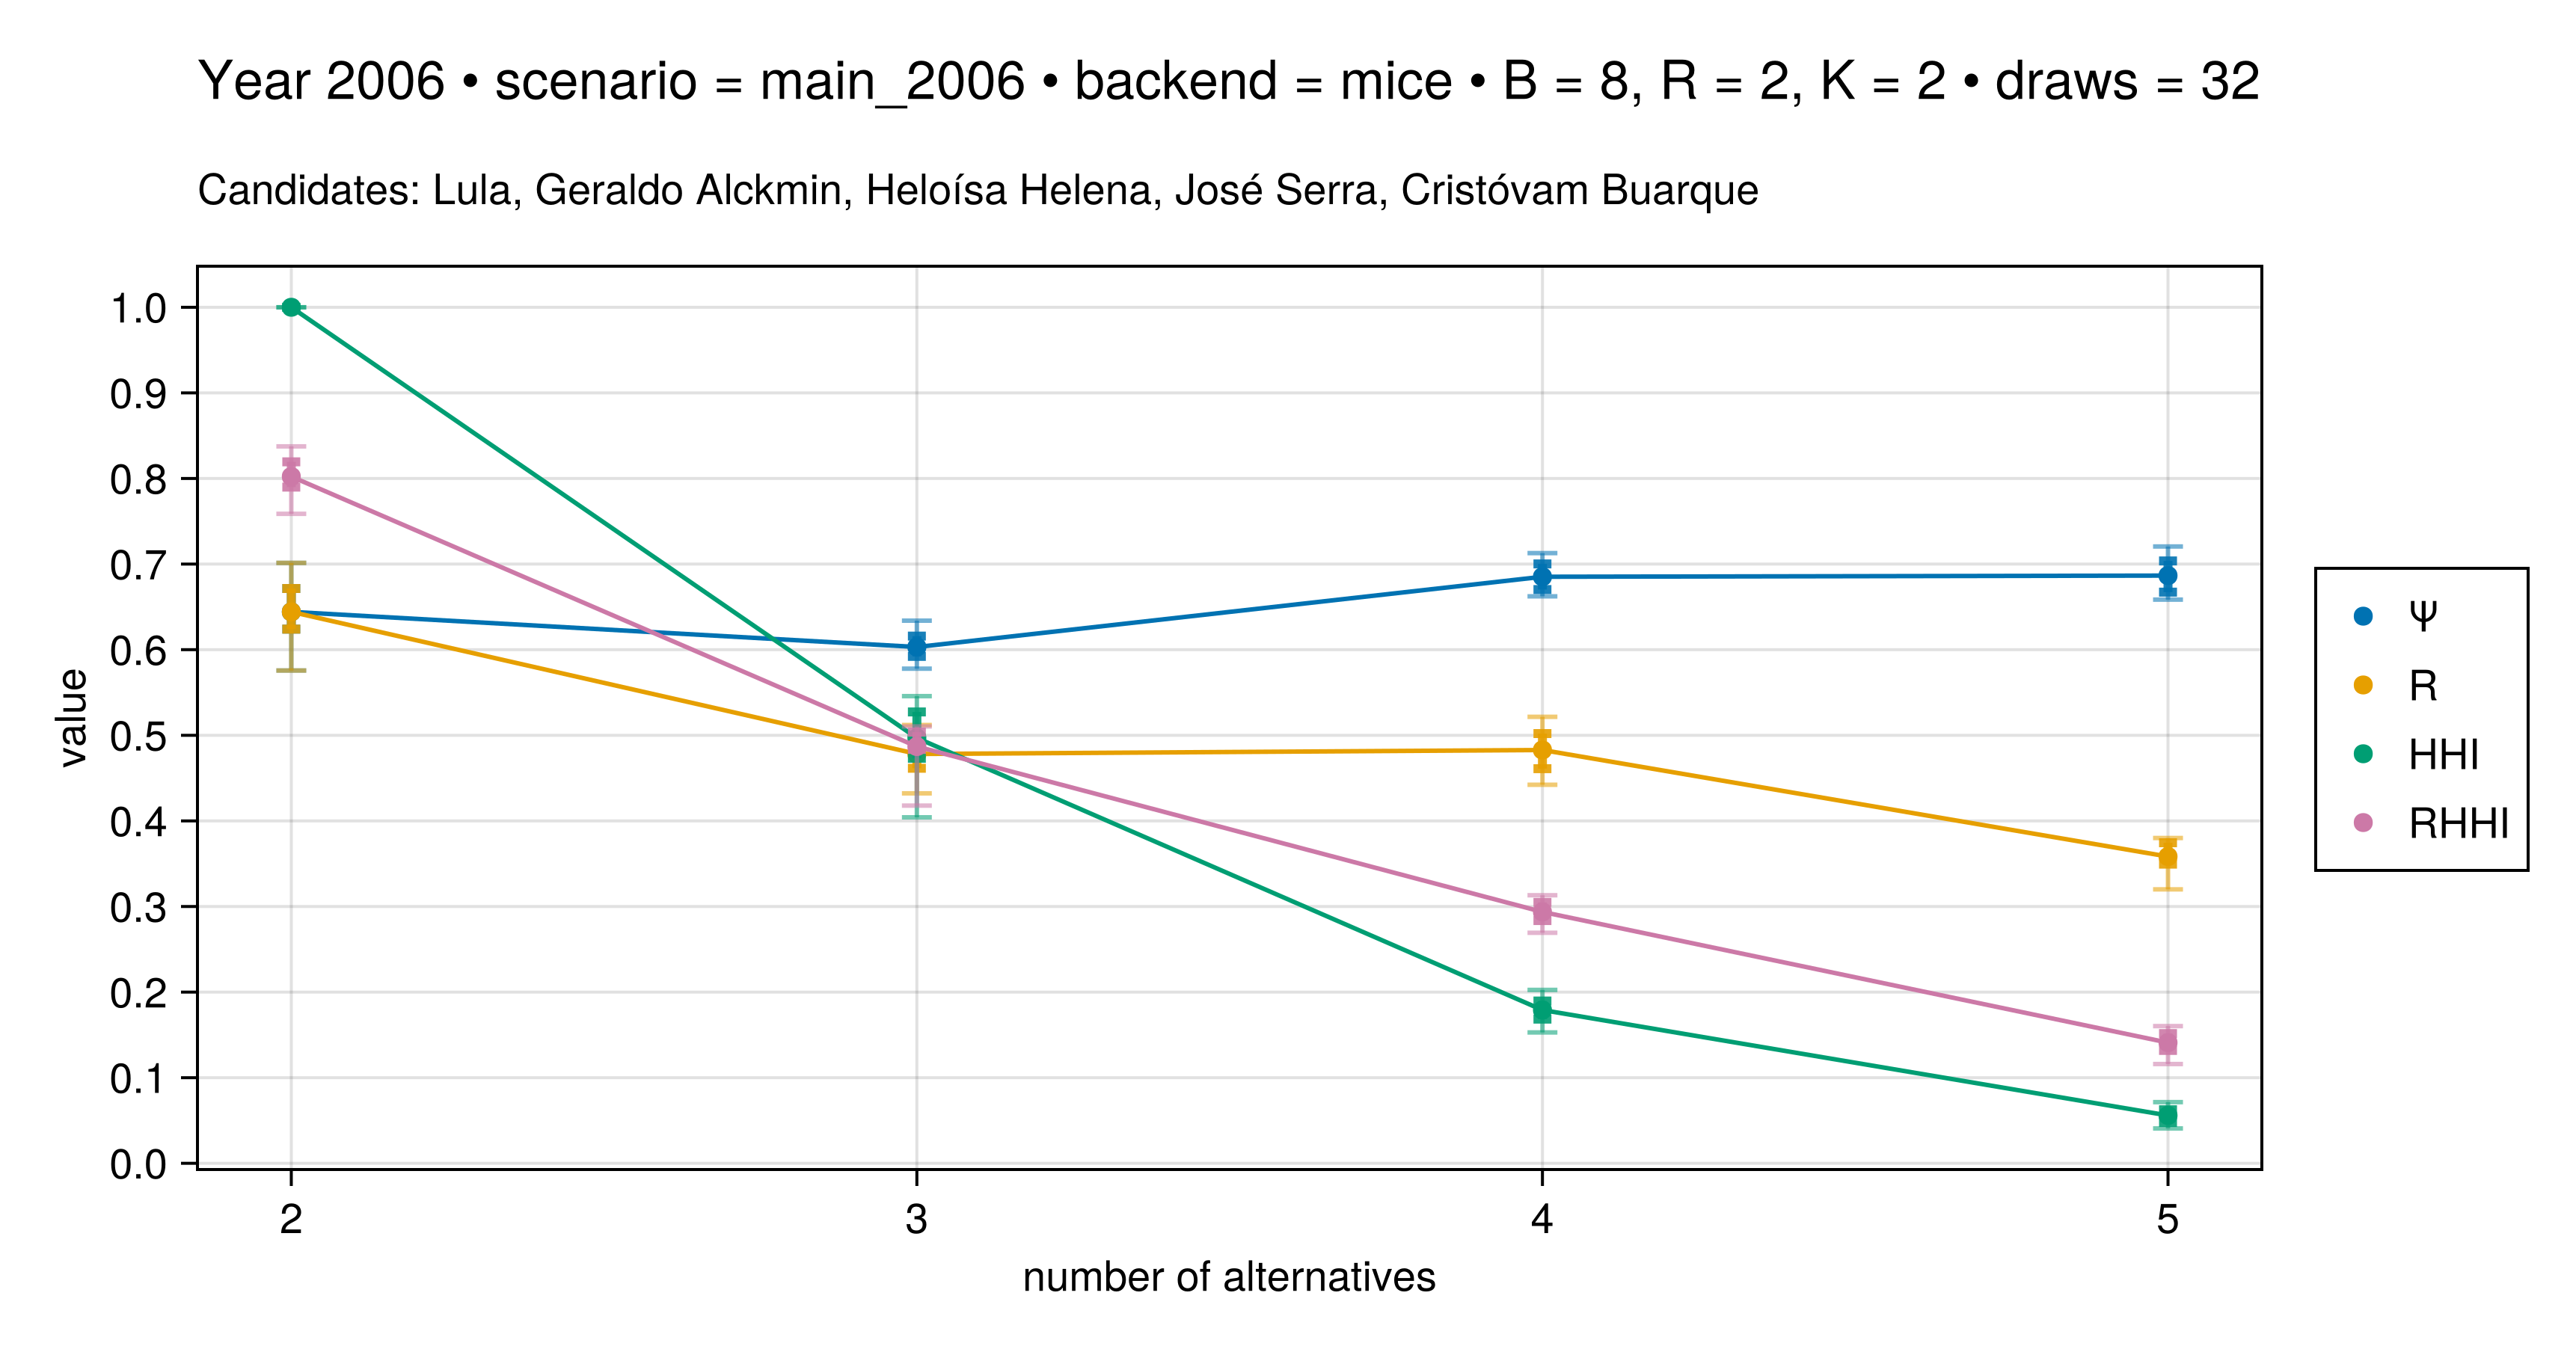
\includegraphics[width=.8\linewidth]{imgs/2006_global_main.png}
  }\par\medskip
  % ----- 2018 -----
  \subcaptionbox{2018\label{fig:globals-2018}}{
    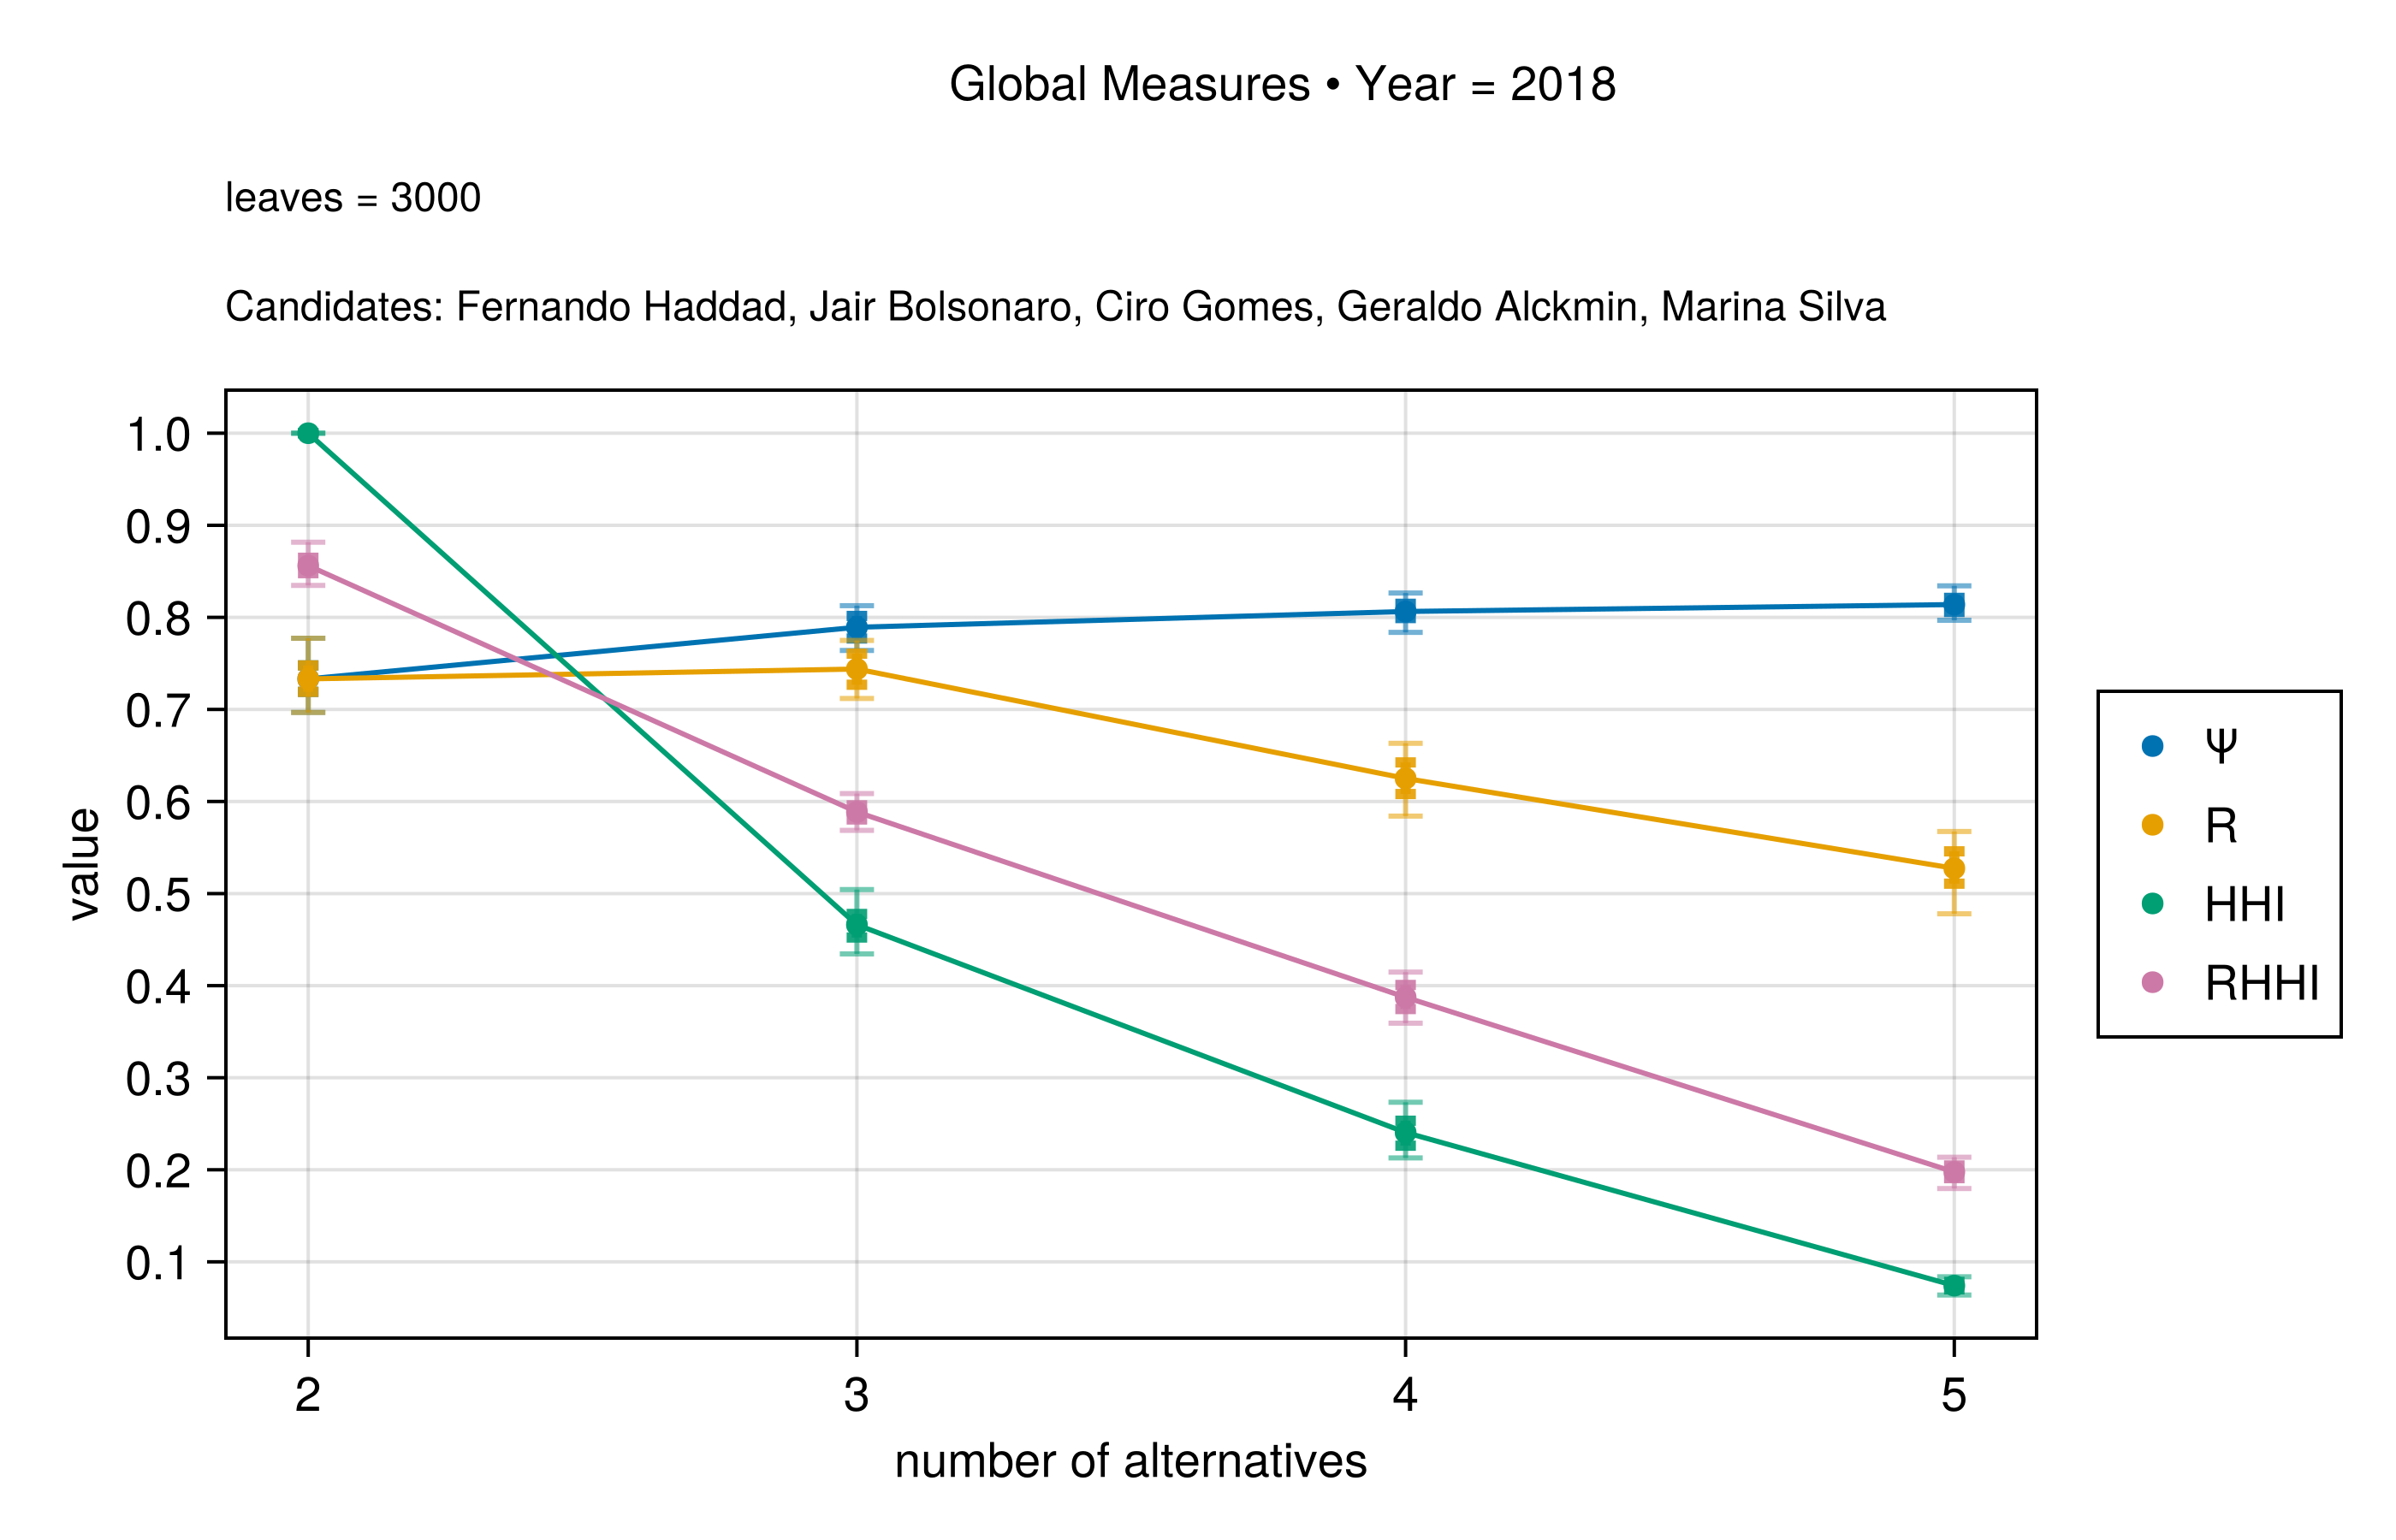
\includegraphics[width=.8\linewidth]{imgs/2018_global_main.png}
  }\par\medskip
  % ----- 2022 -----
  \caption{Evolution of global measures (2006, 2018)}
  \label{fig:globals-evolution}
\end{figure}





\subsection{Results}

% Figure~\ref{fig:globals-evolution} presents the median values\footnote{All global measure plots show median values with quartile bands, while the group measure plots show medians.} of the global measures for the candidate sets analyzed in 2006, 2018, and 2022, varying the number of alternatives \(m\). The candidates appear in the order in which they were included in each scenario. The first mechanical pattern is that \(\kappa=1\) whenever \(m=2\). With only two alternatives, there is only one possible reversal field, \(A \succ B\) versus \(B \succ A\). Hence all reversal mass is necessarily concentrated in that field. For the same reason, \(\Psi\) and \(R\) coincide when \(m=2\), as shown in Appendix~\ref{sec:appendixB}. Since \(RHHI=\sqrt{R\cdot \kappa}\), it follows that \(RHHI=\sqrt{R}\) in the binary case and therefore exceeds \(\Psi=R\) whenever \(0<R<1\). Once \(m\geq 3\), however, the measures separate because reversal can be distributed across multiple opposed ranking pairs.

% The first substantive pattern is the temporal increase in pairwise antagonism. In 2006, \(\Psi\) is already moderate to high, beginning around \(0.64\) for the Lula--Alckmin comparison, falling slightly when Heloísa Helena is added, and then rising to approximately \(0.68\) or \(0.69\) when José Serra and Cristovam Buarque enter the candidate set. In 2018, \(\Psi\) is higher at every comparable value of \(m\): it begins around \(0.74\) for Haddad and Bolsonaro and rises to approximately \(0.81\) for \(m=4\) and \(m=5\). In 2022, \(\Psi\) is higher still. It is around \(0.92\) from \(m=2\) through \(m=4\), declining only slightly to about \(0.89\) at \(m=5\). Thus, according to \(\Psi\), pairwise antagonism increases sharply across the three waves, and by 2022 it remains high even after moving beyond the binary Lula--Bolsonaro comparison.

% However, \(\Psi\) alone does not describe the structure of the profile. It summarizes average pairwise opposition, but it does not say whether the underlying ranking profile is organized around a small number of mutually reversed rankings or dispersed across many ranking configurations. This is why \(R\), \(\kappa\), and \(RHHI\) have to be read together. The measure \(R\) captures the fraction of the profile involved in exact reversal pairs; \(\kappa\) captures how concentrated that reversal mass is across reversal fields; and \(RHHI\) combines the two. A profile can therefore have high \(\Psi\) but lower \(RHHI\) if pairwise antagonism is distributed across many rankings rather than concentrated in a few opposed rankings.

% In 2006, this distinction is especially visible. Exact reversal mass \(R\) is about \(0.64\) at \(m=2\), falls to about \(0.48\) at \(m=3\), remains near \(0.48\) at \(m=4\), and then declines to roughly \(0.36\) at \(m=5\). The concentration component falls even more sharply: \(HHI\) drops from \(1\) at \(m=2\) to about \(0.52\) at \(m=3\), about \(0.18\) at \(m=4\), and about \(0.05\) at \(m=5\). As a result, \(RHHI\) declines from about \(0.80\) in the binary comparison to about \(0.49\), \(0.29\), and \(0.14\) as the candidate set expands. The interpretation is not that conflict disappears in 2006. Rather, as the profile is represented over a richer ranking space, exact reversal mass becomes increasingly diffuse.

% The 2018 profile is more conflictual than the 2006 profile. \(R\) is about \(0.74\) at \(m=2\), remains around \(0.75\) at \(m=3\), and then declines to approximately \(0.64\) and \(0.54\) at \(m=4\) and \(m=5\). These values are consistently above the 2006 values at comparable candidate-set sizes. The concentration component again falls with \(m\), from \(1\) at \(m=2\) to roughly \(0.47\), \(0.25\), and \(0.08\). Consequently, \(RHHI\) falls from about \(0.86\) to \(0.59\), \(0.39\), and \(0.20\). The important point is that the decline in \(RHHI\) with \(m\) is compatible with a more conflictual profile. Compared with 2006, 2018 has higher pairwise antagonism, higher exact reversal mass, and higher reversal-concentration composites, but the opposition is still distributed over multiple reversal fields once more than two candidates are considered.

% The 2022 profile displays the strongest global pattern. Exact reversal mass is about \(0.92\) at \(m=2\), remains near \(0.90\) at \(m=3\), is still around \(0.84\) at \(m=4\), and only then declines to approximately \(0.65\) at \(m=5\). This is a major difference from the earlier waves: reversal mass remains high even after the candidate set moves beyond the two leading candidates. \(\kappa\) still declines mechanically as the ranking space expands, from \(1\) at \(m=2\) to about \(0.67\), \(0.33\), and \(0.14\). But because \(R\) remains high, the composite \(RHHI\) also remains much higher than in the previous years: approximately \(0.96\), \(0.78\), \(0.53\), and \(0.30\) from \(m=2\) to \(m=5\). In profile-space terms, 2022 combines very high pairwise antagonism with substantial exact reversal mass and comparatively stronger concentration of that reversal mass.

% The effective number of reversal pairs, \(1/\kappa\), makes the same point in more interpretable terms. With three alternatives, the theoretical maximum number of reversal pairs is \(3\). The effective number is about \(1.9\) in 2006, \(2.1\) in 2018, and \(1.5\) in 2022. Thus, at \(m=3\), 2022 has the largest reversal mass but the smallest effective number of reversal fields. Its opposition is therefore both stronger and more concentrated. With four alternatives, the theoretical maximum is \(12\), while the effective numbers are approximately \(5.6\), \(4.0\), and \(3.0\) in 2006, 2018, and 2022. With five alternatives, the theoretical maximum is \(60\), while the effective numbers are roughly \(18\), \(13\), and \(7\). The expansion of the candidate set necessarily opens many possible reversal fields, but the 2022 profile uses fewer of them effectively.

% This decomposition clarifies why \(\Psi\) and \(RHHI\) should not be interpreted as competing measures of the same object. \(\Psi\) captures the intensity of pairwise antagonism. \(RHHI\) captures reversal mass weighted by its concentration across exact opposite rankings. The fact that \(\Psi\) remains high while \(RHHI\) declines with \(m\) means that pairwise antagonism can be intense even when exact reversal is distributed across a large ranking space. Conversely, the fact that 2022 has higher \(RHHI\) than 2006 and 2018 at comparable values of \(m\) means that its antagonism is not merely a marginal pairwise phenomenon. It is also more organized in the profile space.


Figure~\ref{fig:globals-evolution} presents the median values\footnote{All
global measure plots show median values with quartile bands, while the group
measure plots show medians.} of the global measures for the candidate sets
analyzed in 2006, 2018, and 2022, varying the number of alternatives \(m\). The
candidates appear in the order in which they were included in each scenario.
The binary case must be read separately. When \(m=2\), there is only one
possible reversal field, \(A \succ B\) versus \(B \succ A\). Hence
\(\kappa=1\), \(\Psi=R\), and \(RHHI=\sqrt{R}\). In this case, a close binary
comparison mechanically appears as concentrated opposition because there is no
larger ranking space in which reversal mass can disperse. Once \(m\geq 3\), the
measures separate: pairwise antagonism, exact reversal mass, and reversal
concentration become distinct features of the profile.

The first substantive pattern is the temporal increase in pairwise antagonism.
In 2006, \(\Psi\) is already moderate to high, ranging from about \(0.64\) to
about \(0.69\) across candidate-set sizes. In 2018, it is higher at every
comparable value of \(m\), rising from about \(0.73\) in the binary comparison
to roughly \(0.81\) for larger candidate sets. In 2022, it is higher still:
\(\Psi\) is about \(0.90\) at \(m=2\), remains around \(0.91\)--\(0.92\) for
\(m=3\) and \(m=4\), and then declines to about \(0.88\) at \(m=5\). Thus,
the relevant change is not the emergence of antagonism from a neutral baseline.
It is the intensification of an already nontrivial level of pairwise dissent,
with 2022 standing out even after the analysis moves beyond the Lula--Bolsonaro
comparison.

\begin{figure}
  \centering
    {
    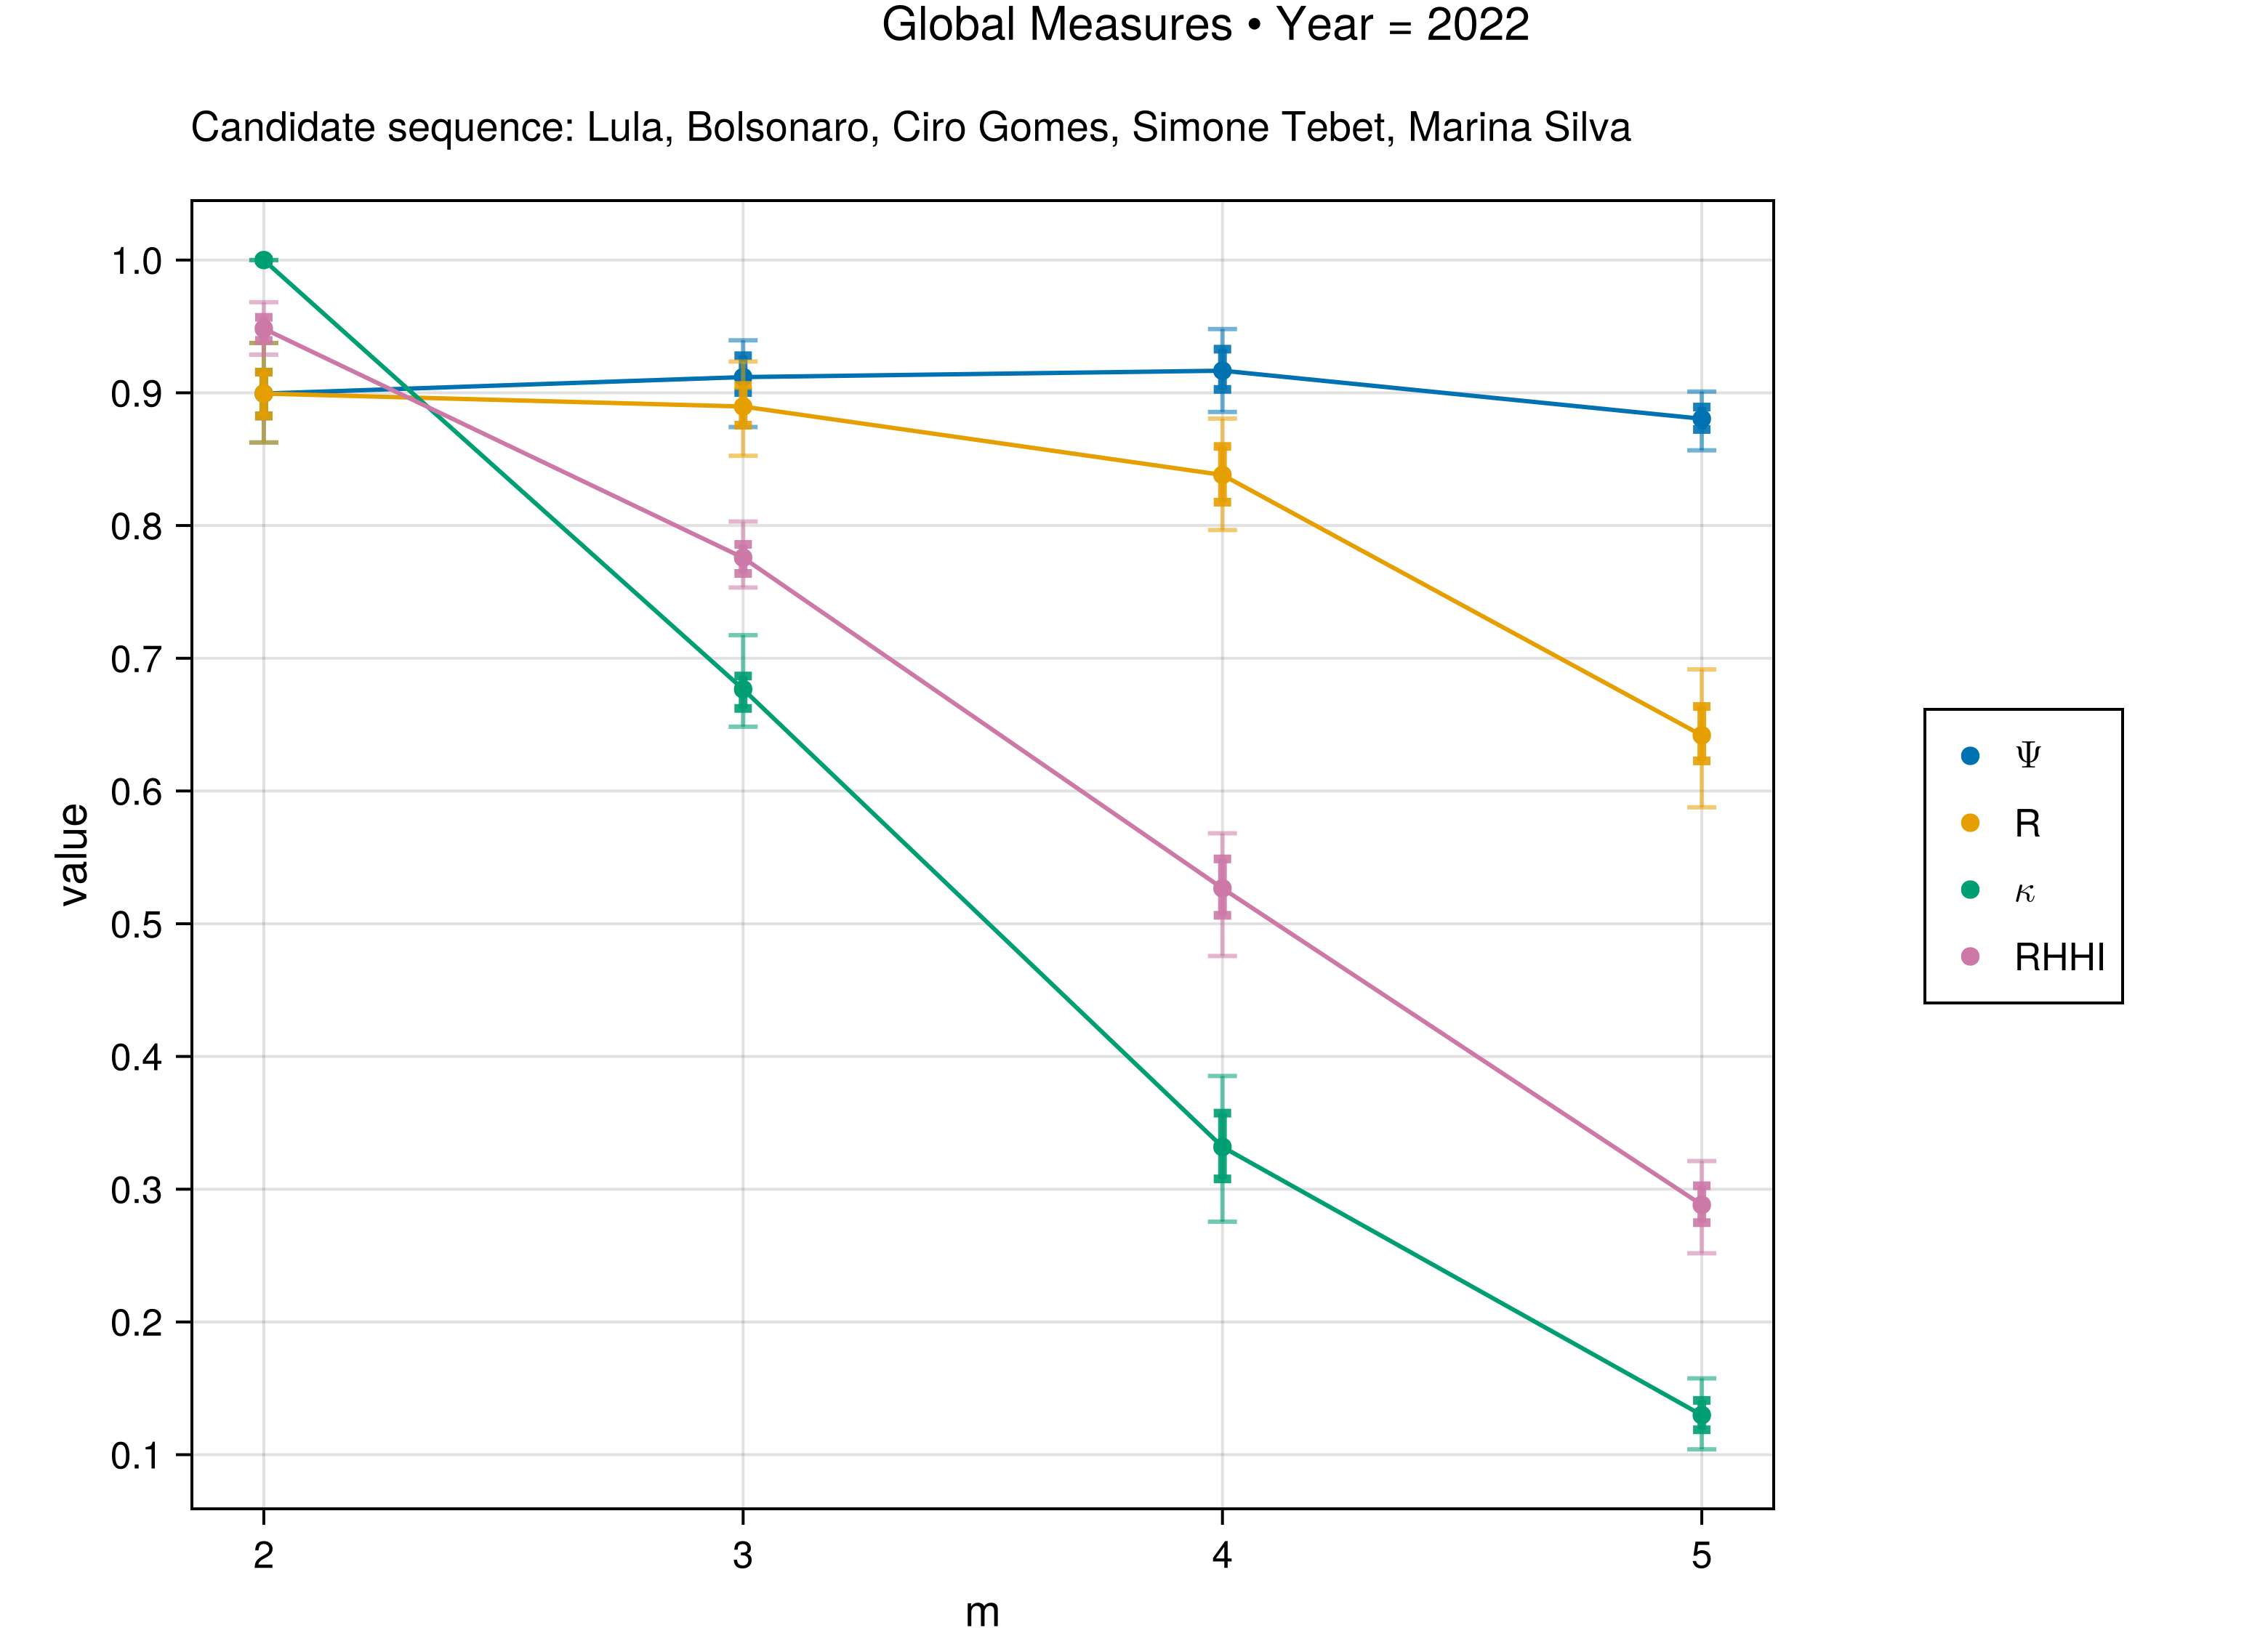
\includegraphics[width=.8\linewidth]{imgs/2022_global_main.png}
  }

\end{figure}

However, \(\Psi\) does not describe the structure of that dissent. It summarizes
average pairwise opposition, but it does not show whether the profile is
organized around a small number of opposed rankings or dispersed across many
ranking configurations. This is why \(R\), \(\kappa\), and \(RHHI\) have to be
read together. \(R\) measures how much of the profile lies in exact reversal
pairs; \(\kappa\) measures how concentrated that reversal mass is across
reversal fields; and \(RHHI\) combines reversal mass with its concentration.

This decomposition changes the interpretation of the temporal pattern. In
2006, exact reversal mass falls as the candidate set expands, and the
concentration component falls even more sharply. \(RHHI\) therefore declines
from about \(0.80\) in the binary comparison to about \(0.14\) at \(m=5\). This
does not mean that conflict disappears, but that, once the profile is
represented in a richer ranking space, exact opposition becomes diffuse. The
2018 profile is more conflictual: \(R\) remains above the 2006 values at
comparable candidate-set sizes, and \(RHHI\) is also higher. But the same
structural pattern remains: as \(m\) grows, opposition is distributed across
multiple reversal fields rather than concentrated in a single opposed pair of
rankings.

The 2022 profile is different in degree and structure. Exact reversal mass
remains high even after additional candidates enter the ranking set: \(R\) is
about \(0.90\) at \(m=2\), near \(0.89\) at \(m=3\), around \(0.84\) at
\(m=4\), and still about \(0.64\) at \(m=5\). Although \(\kappa\) declines as
the ranking space expands, it remains higher than in the earlier waves at
comparable values of \(m\). As a result, \(RHHI\) remains substantially above
the 2006 and 2018 levels, reaching about \(0.29\) at \(m=5\). In profile-space
terms, 2022 combines very high pairwise antagonism with substantial exact
reversal mass and comparatively stronger concentration of that reversal mass.

The global measures therefore do not support a simple binary-polarization
interpretation. Binary comparisons mechanically force all reversal into one
field, while richer candidate sets reveal whether antagonism remains organized
or disperses across the ranking space. The observed pattern is increasing
antagonism with increasing compression: by 2022, more of the profile is involved
in exact opposition, and that opposition is carried by fewer effective regions
of the ranking space than in earlier waves.



\begin{figure}[htbp]
    \hspace*{-1cm} 
 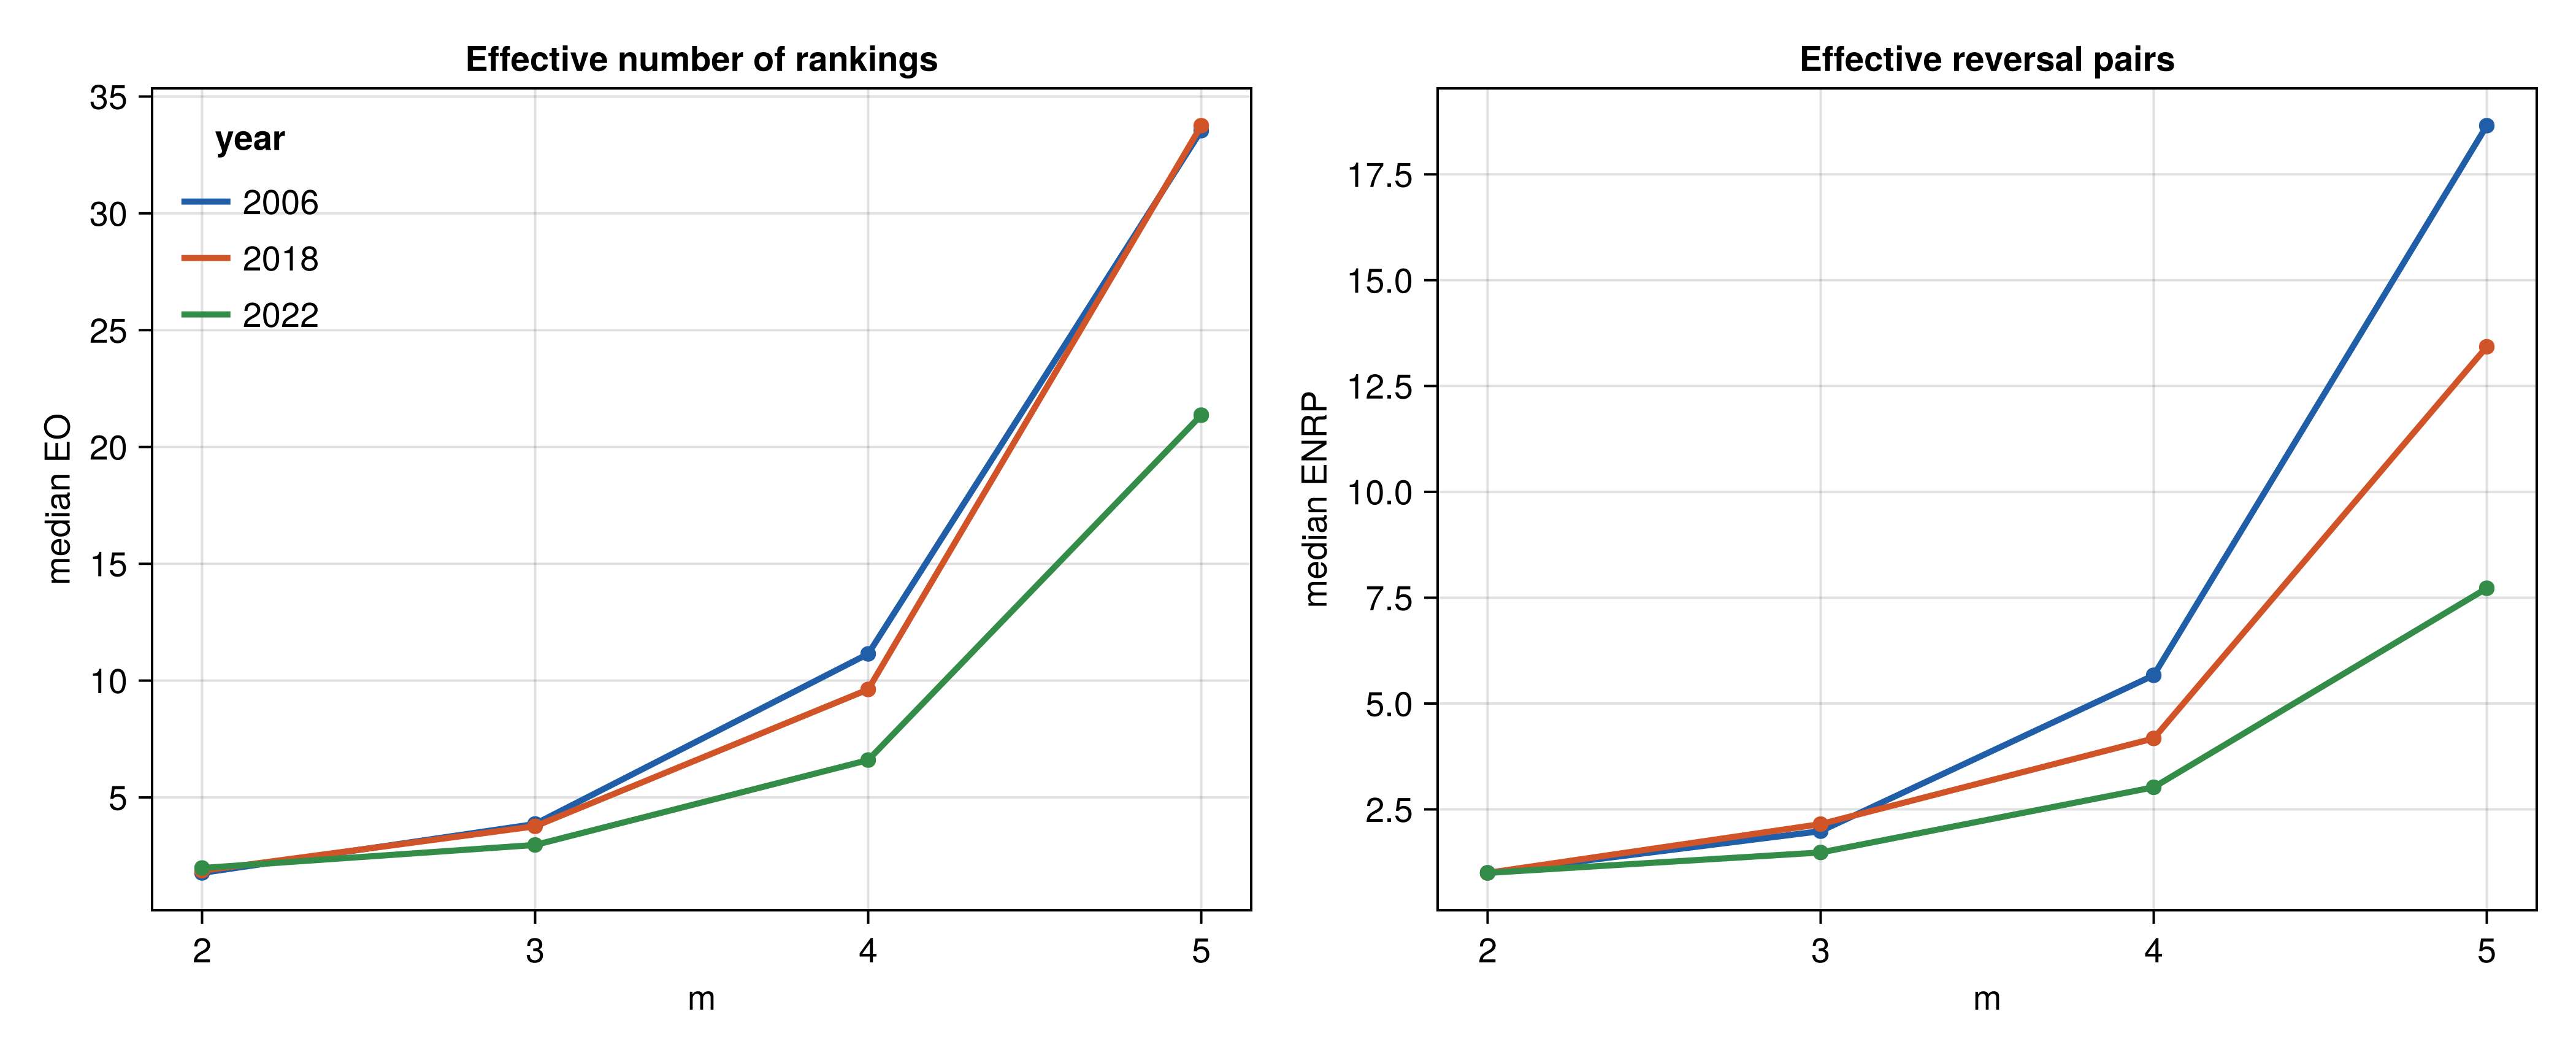
\includegraphics[ width=1.1\textwidth, keepaspectratio]{imgs/effective_rankings_evolution_1x2.png}
  \caption{Compression of profiles according to EO and ENRP}
  \label{fig:enrp-stuff}
\end{figure}

After the global indices, Figure~\ref{fig:enrp-stuff} adds a diagnostic view of the structure of the observed profile. The left panel reports the effective number of rankings, while the right panel reports the effective number of reversal pairs. Together, they show how much of the ranking space is effectively occupied and how diffuse or concentrated the exact-reversal structure is.

The first result is that the effective support naturally expands sharply with \(m\), but not uniformly across years. At \(m=2\), the three elections are nearly indistinguishable: the profile is close to the two-ranking limit, and there is only one possible reversal pair. As \(m\) increases, however, the years separate. In 2006 and 2018, the effective number of rankings rises steeply, reaching similar levels at \(m=5\): \(33.54\) effective rankings in 2006 and \(33.75\) in 2018. In 2022, by contrast, the profile remains much more compressed, reaching only \(21.36\) effective rankings. Thus, although the formal ranking space grows factorially with \(m\), the observed 2022 profile occupies a smaller effective subspace.

The reversal-pair diagnostic sharpens this contrast. By \(m=5\), 2006 has \(18.65\) effective reversal pairs and 2018 has \(13.43\), while 2022 has only \(7.72\). This indicates that the exact-reversal mass in 2022 is more concentrated: opposition is organized through fewer structurally opposed ranking pairs. In 2006 and 2018, reversal mass is more diffuse, spread across a larger set of opposing rankings\footnote{The appendix table reports the same diagnostics numerically.}.



Taken together, the global indices and the effective-support diagnostics suggest that the observed process is not simply a movement from pluralism to two-bloc polarization. Later waves show greater organization of disagreement, especially in 2022, where the ranking space is more compressed and reversal mass is more concentrated. Yet this concentration does not amount to dominance by a single antagonistic reversal pair.

When the choice set is binary (\(m=2\)), the global measures partially
collapse to the normalized pair margin. In this case, a close race, understood
as a small aggregate margin between the two alternatives, is equivalent to high
\(\Psi\) and high \(R\). But the same binary restriction also forces
\(\kappa=1\) and \(ENRP=1\). Hence, any further structure is unidentifiable:
all opposition is concentrated in a single reversal field by construction.
For this reason, reading a narrow electoral margin as ``high polarization,''
as in \textcite[pp.~17--18]{nunes2023biografia}, is misleading. It confuses
a binary margin with the structure of the preference profile.

The point becomes visible as soon as \(m\geq 3\). Once additional alternatives
are admitted, reversal mass can be distributed across multiple opposed
rankings. \(RHHI\) therefore falls relative to the binary case, and
\(ENRP>1\) shows that antagonism does not collapse onto a single divide.
At the same time, the updated results show that this dispersion is not random
fragmentation. In 2022, pairwise antagonism and reversal mass remain high even
for larger candidate sets, while the effective number of reversal fields is
smaller than in the earlier waves. The substantive conclusion is therefore
more precise: binary margins overstate what can be inferred about
polarization, but the multiparty profile reveals a real increase in structured
opposition, especially in 2022.
 




% ---------- 2006 ----------
\begin{figure}[htbp]
  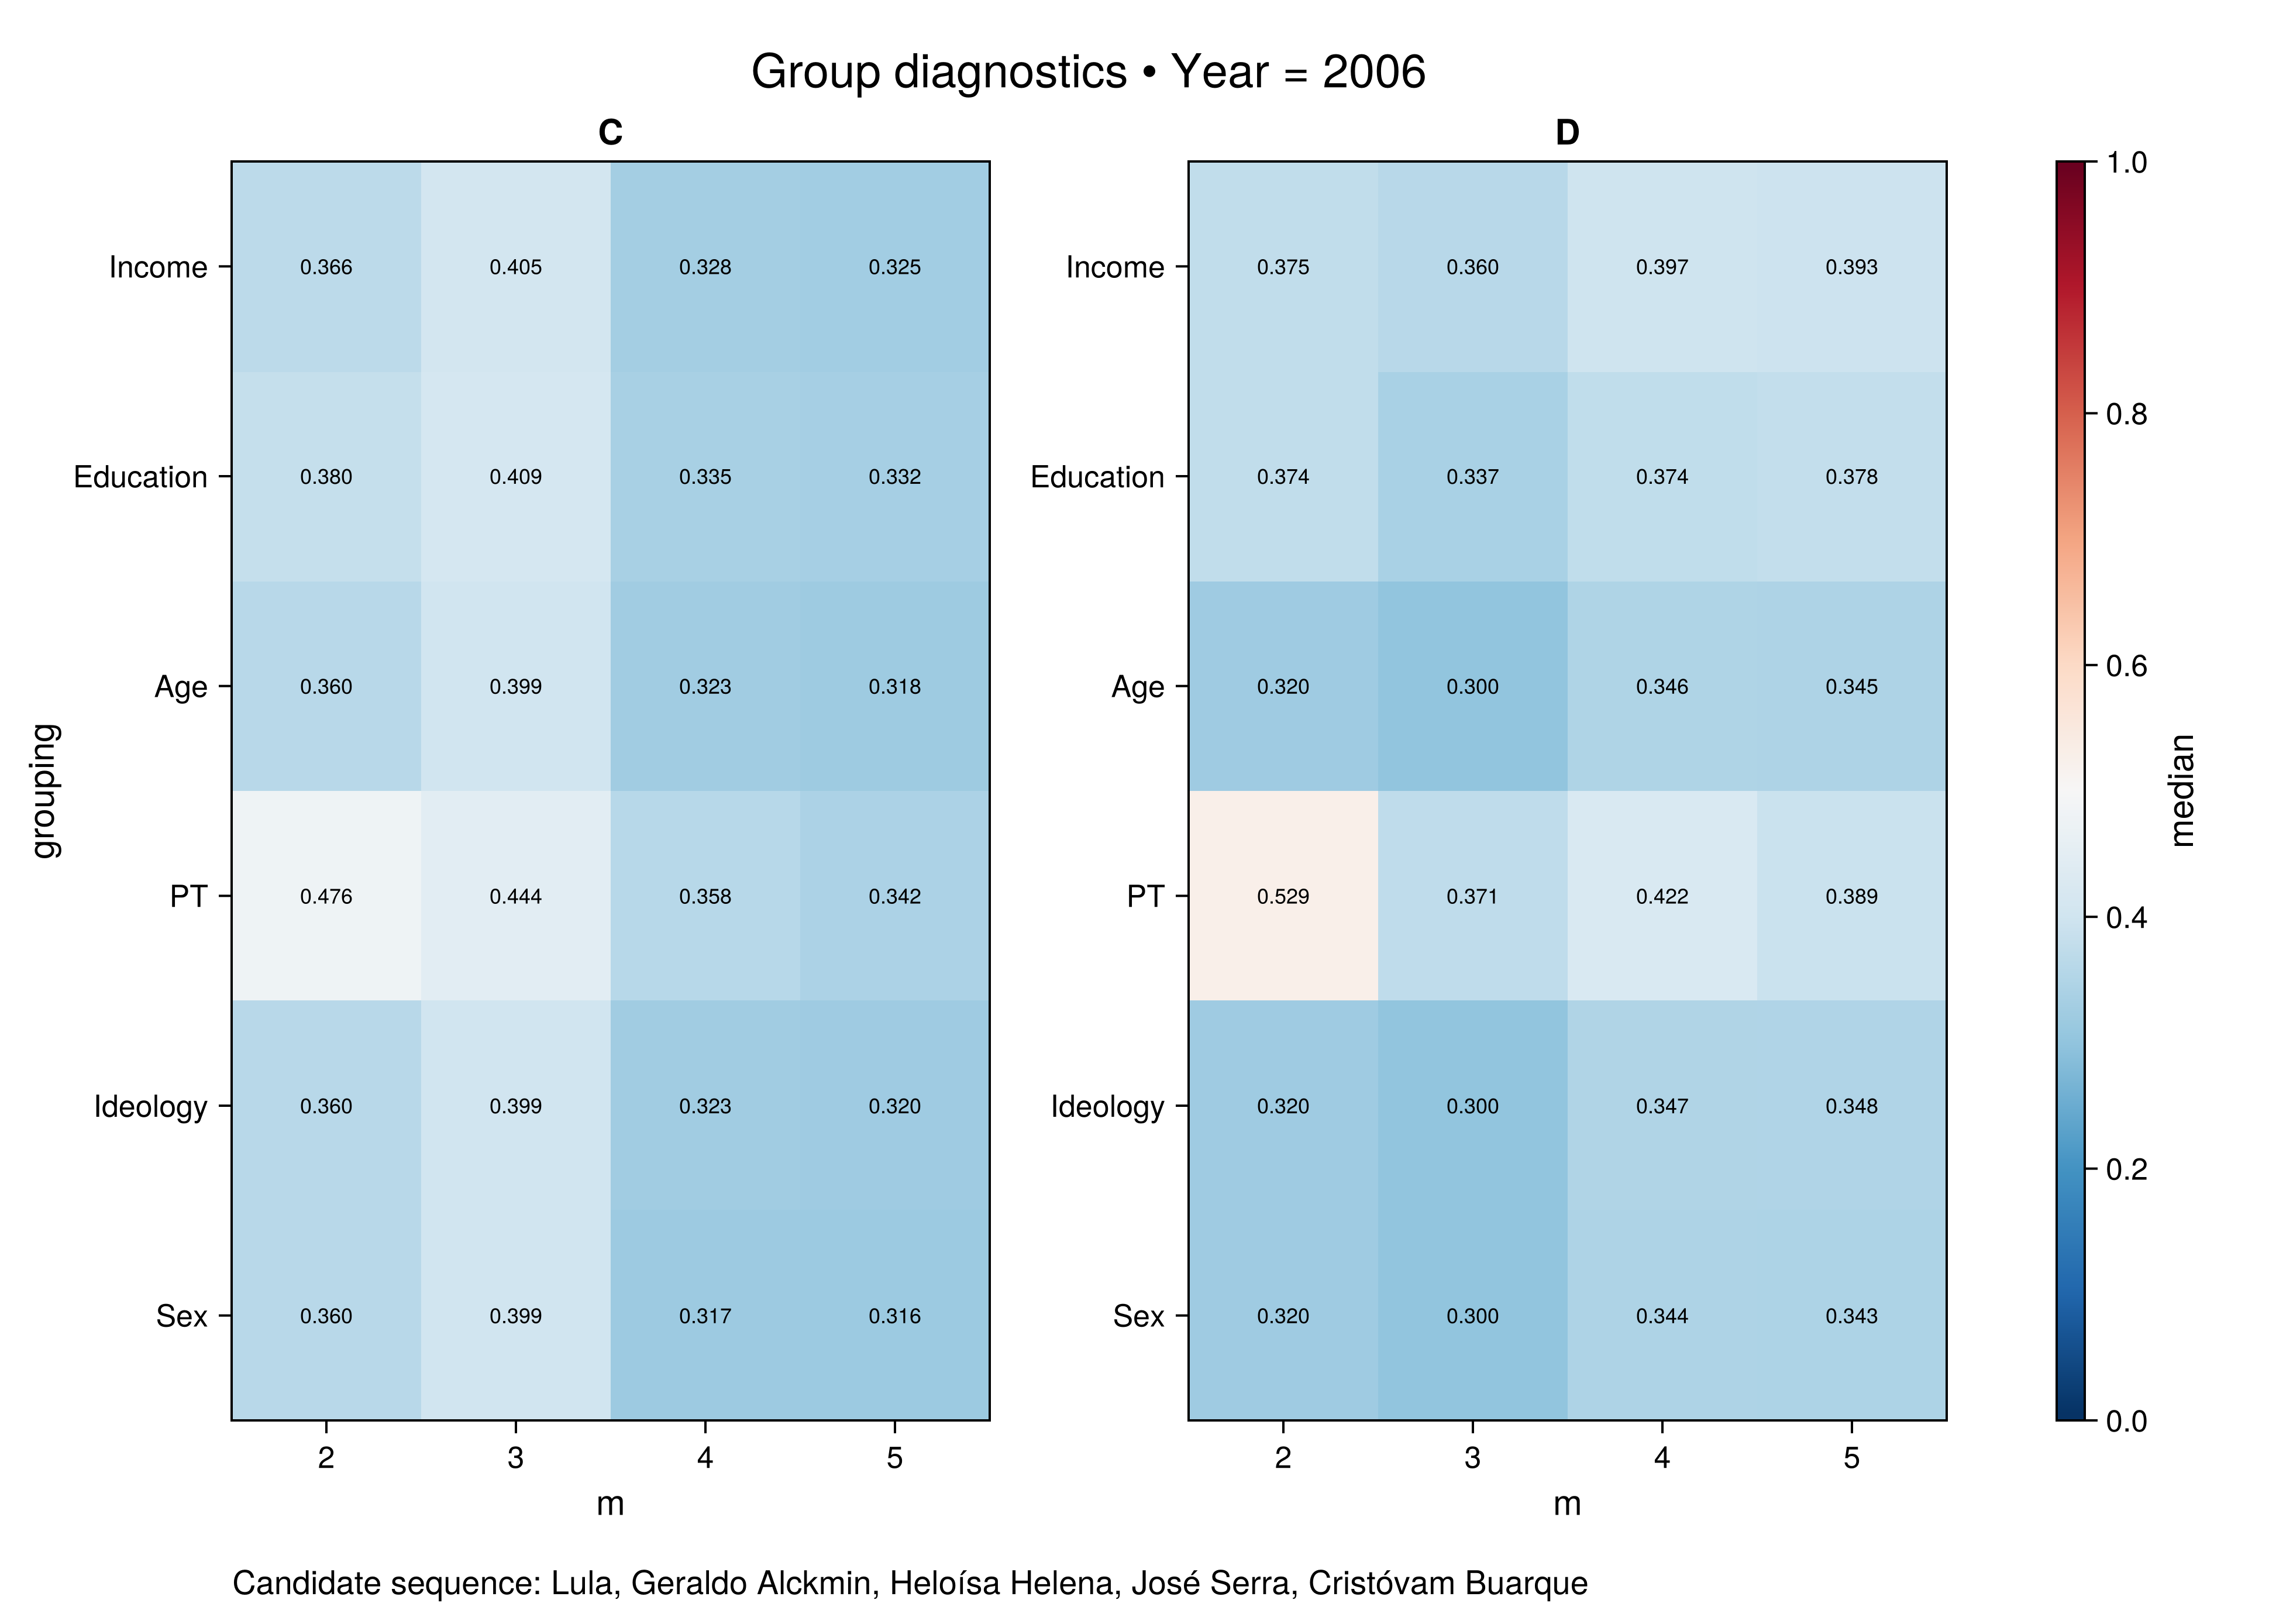
\includegraphics[width=\textwidth,keepaspectratio]{imgs/2006_group_C_D.png}
  \caption{Group diagnostics in 2006: within-group coherence \(C\) and between-group divergence \(D\).}
  \label{fig:group-2006}
\end{figure}

Figure~\ref{fig:group-2006} reports the group-based diagnostics for 2006:
within-group coherence \(C\) and between-group divergence \(D\). The main
result is weak group structuration overall, with PT evaluation as the partial
exception. For most demographic partitions, \(C\) is positive but modest,
usually between about \(0.32\) and \(0.41\), and it declines or remains flat as
the candidate set expands. Their \(D\) values are also moderate, but rarely
distinctive: sex, ideology, and age are especially similar, while education and
income are slightly higher. Thus, these partitions identify some differences in
group consensuses, but they do not organize the profile strongly.

PT evaluation stands out in 2006. It has the highest coherence at \(m=2\),
with \(C \approx 0.47\), and the highest divergence, with \(D \approx 0.53\).
However, this PT-centered structuration weakens as additional candidates enter
the ranking set. By \(m=5\), PT's \(C\) has fallen to about \(0.34\) and
\(D\) to about \(0.39\). Thus, in 2006, PT evaluation structures the binary
comparison, but much less of the richer ranking profile. The other 2006
groupings do not combine high internal coherence with high external divergence,
so the observed demographic partitions do not generate compact and mutually
distant blocs.

% ---------- 2018 ----------
\begin{figure}[htbp]
  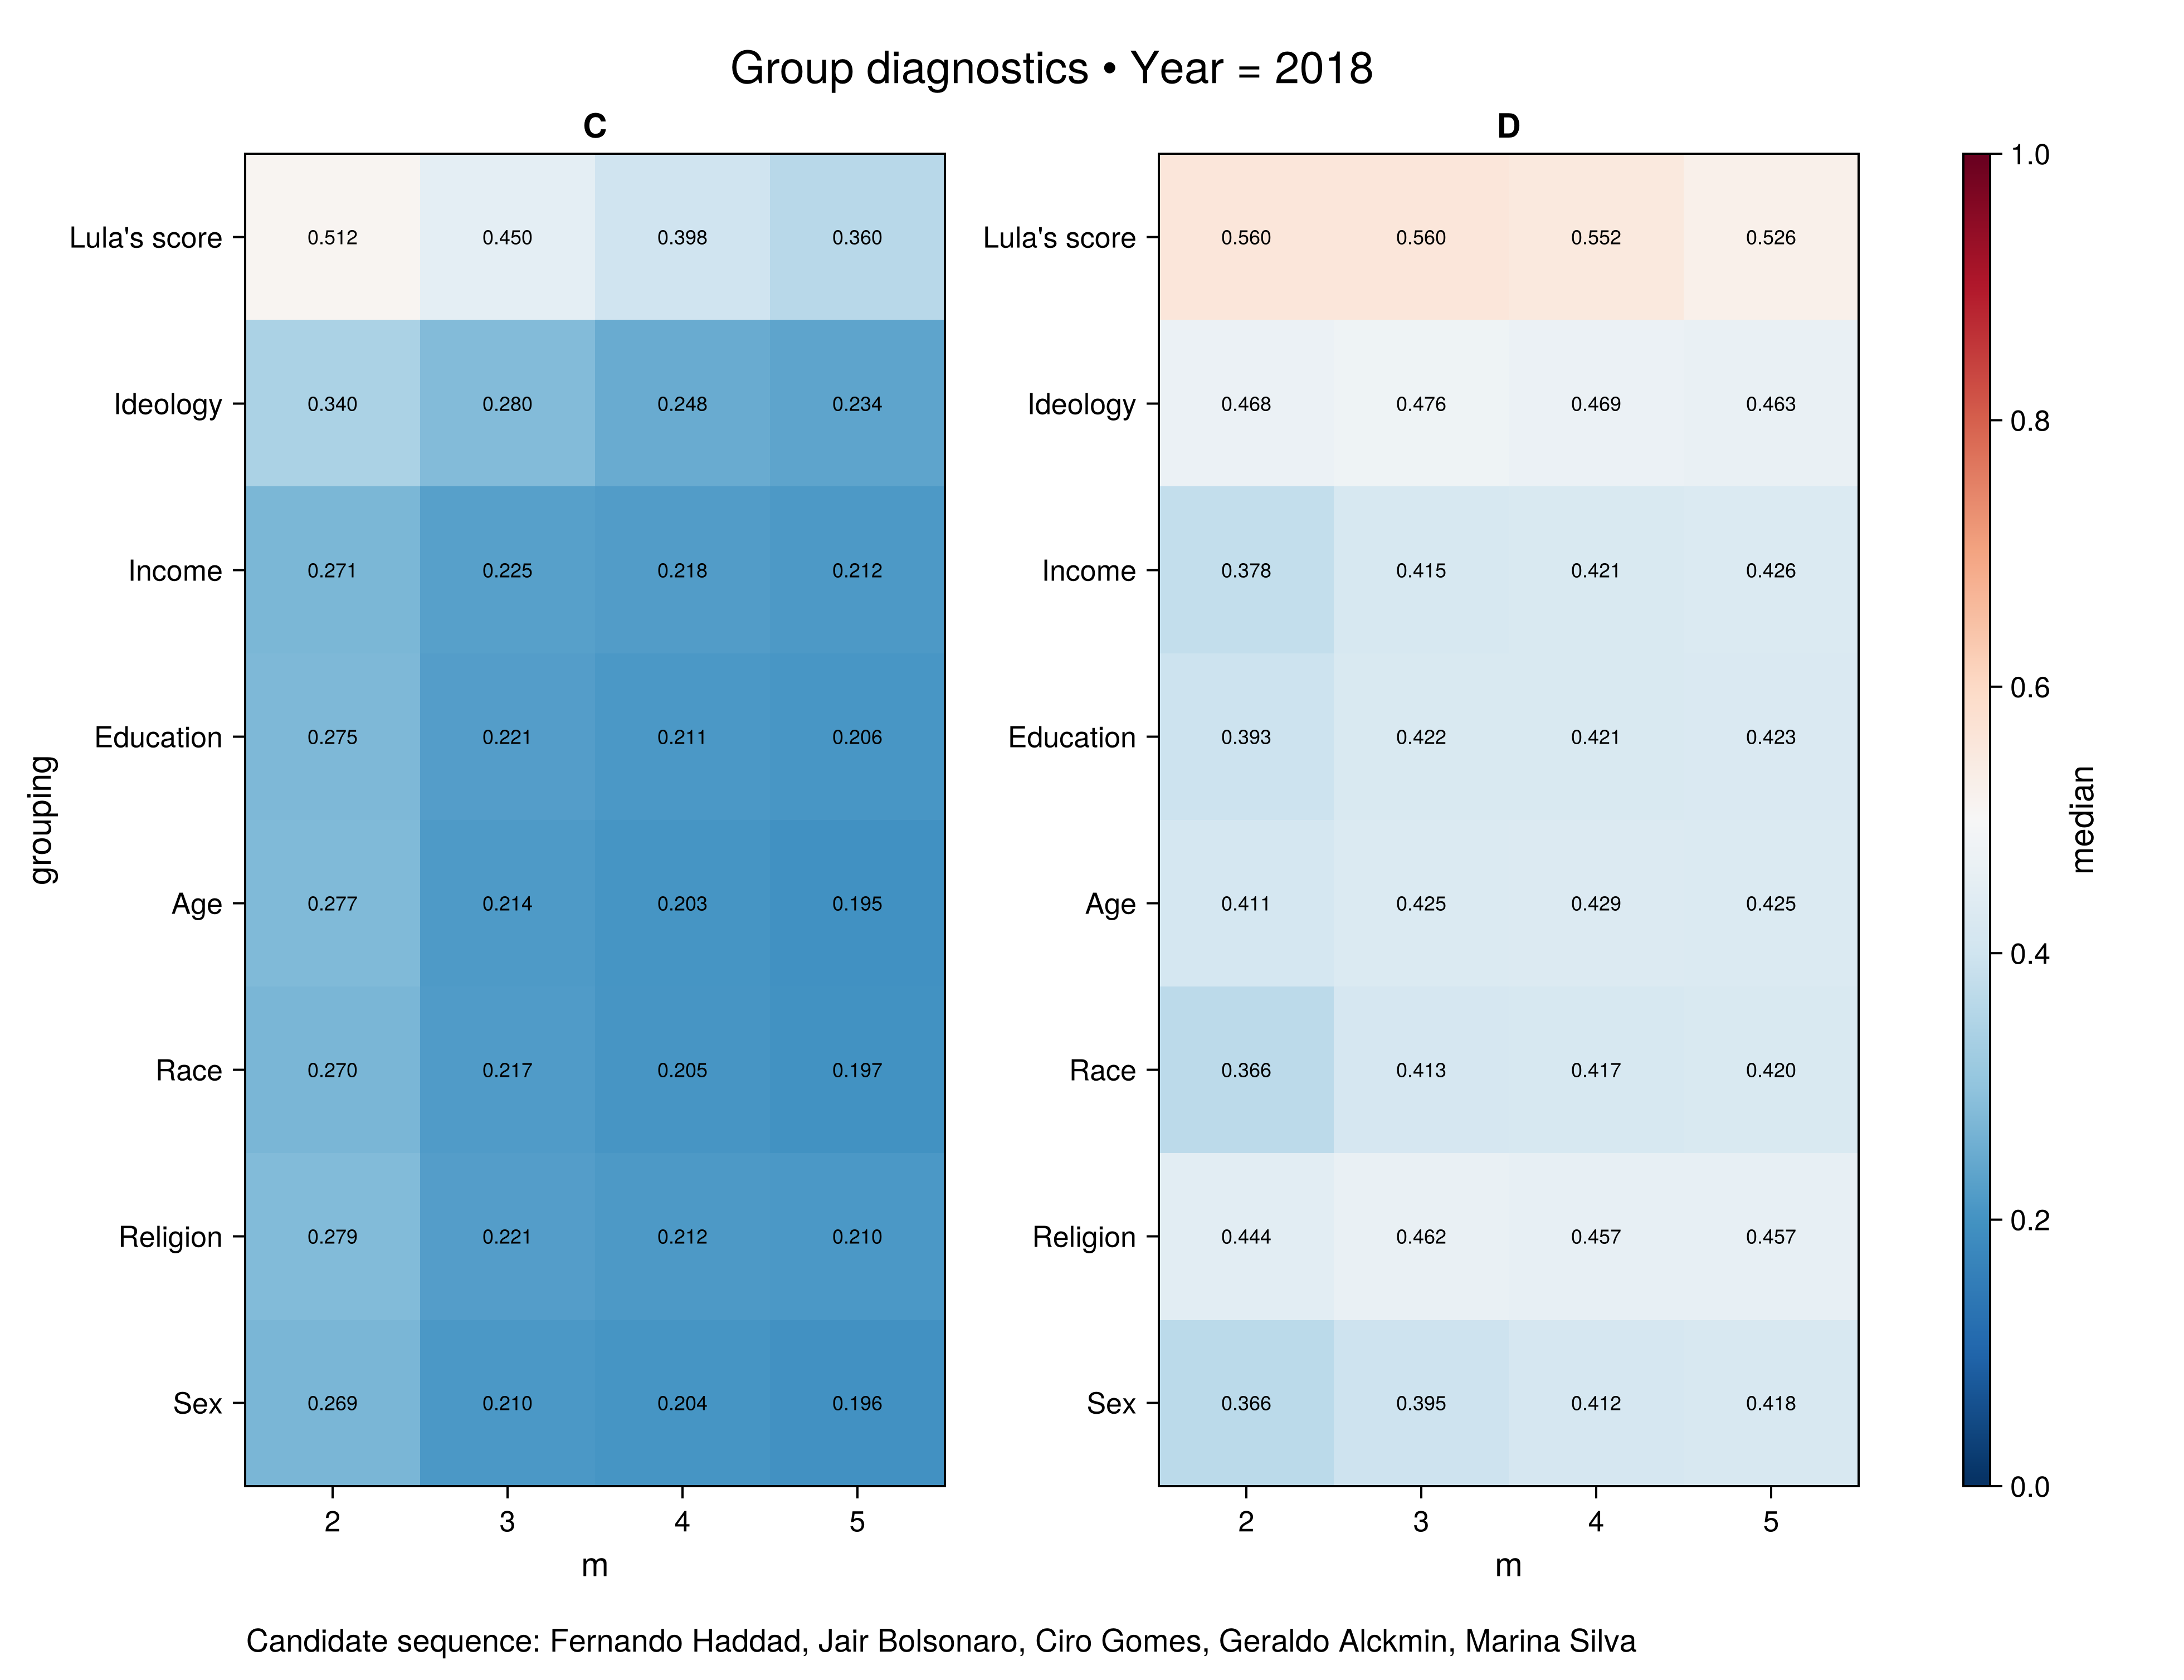
\includegraphics[width=\textwidth,keepaspectratio]{imgs/2018_group_C_D.png}
  \caption{Group diagnostics in 2018: within-group coherence \(C\) and between-group divergence \(D\).}
  \label{fig:group-2018}
\end{figure}

Figure~\ref{fig:group-2018} shows a different pattern. The PT evaluation
variable is not used because of the very high number of missing responses in
2018.\footnote{Approximately 1500 out of 2500 responses are missing.} Instead,
the relevant political grouping is respondents' score for Lula. This variable
dominates the 2018 group diagnostics. It has the highest within-group
coherence, beginning at \(C \approx 0.51\) for \(m=2\) and declining to
\(C \approx 0.36\) by \(m=5\). It also has the highest between-group
divergence, from \(D \approx 0.56\) at \(m=2\) to \(D \approx 0.53\) at
\(m=5\). The 2018 profile is therefore not simply more conflictual than 2006;
among the tested partitions, Lula score is the clearest grouping associated
with coherent and externally divergent subprofiles.

Among the groupings examined in 2018, ideology is the second most informative
political partition. It is consistently above the demographic baselines, with
\(C\) around \(0.34\) at \(m=2\) and \(0.24\) at \(m=5\), while \(D\) remains
around \(0.47\). Religion also has relatively high \(D\), near \(0.45\) to
\(0.47\), but its coherence is weaker than Lula score. Compared with 2006, the
2018 demographic partitions show lower coherence and higher divergence. Sex,
race, income, education, and age all have relatively low \(C\), mostly near
\(0.20\) to \(0.28\), while their \(D\) values often lie around \(0.39\) to
\(0.43\). These groups are internally less cohesive than comparable partitions
in 2006, even when their fitted consensuses are somewhat farther apart.

% ---------- 2022 ----------
\begin{figure}[htbp]
  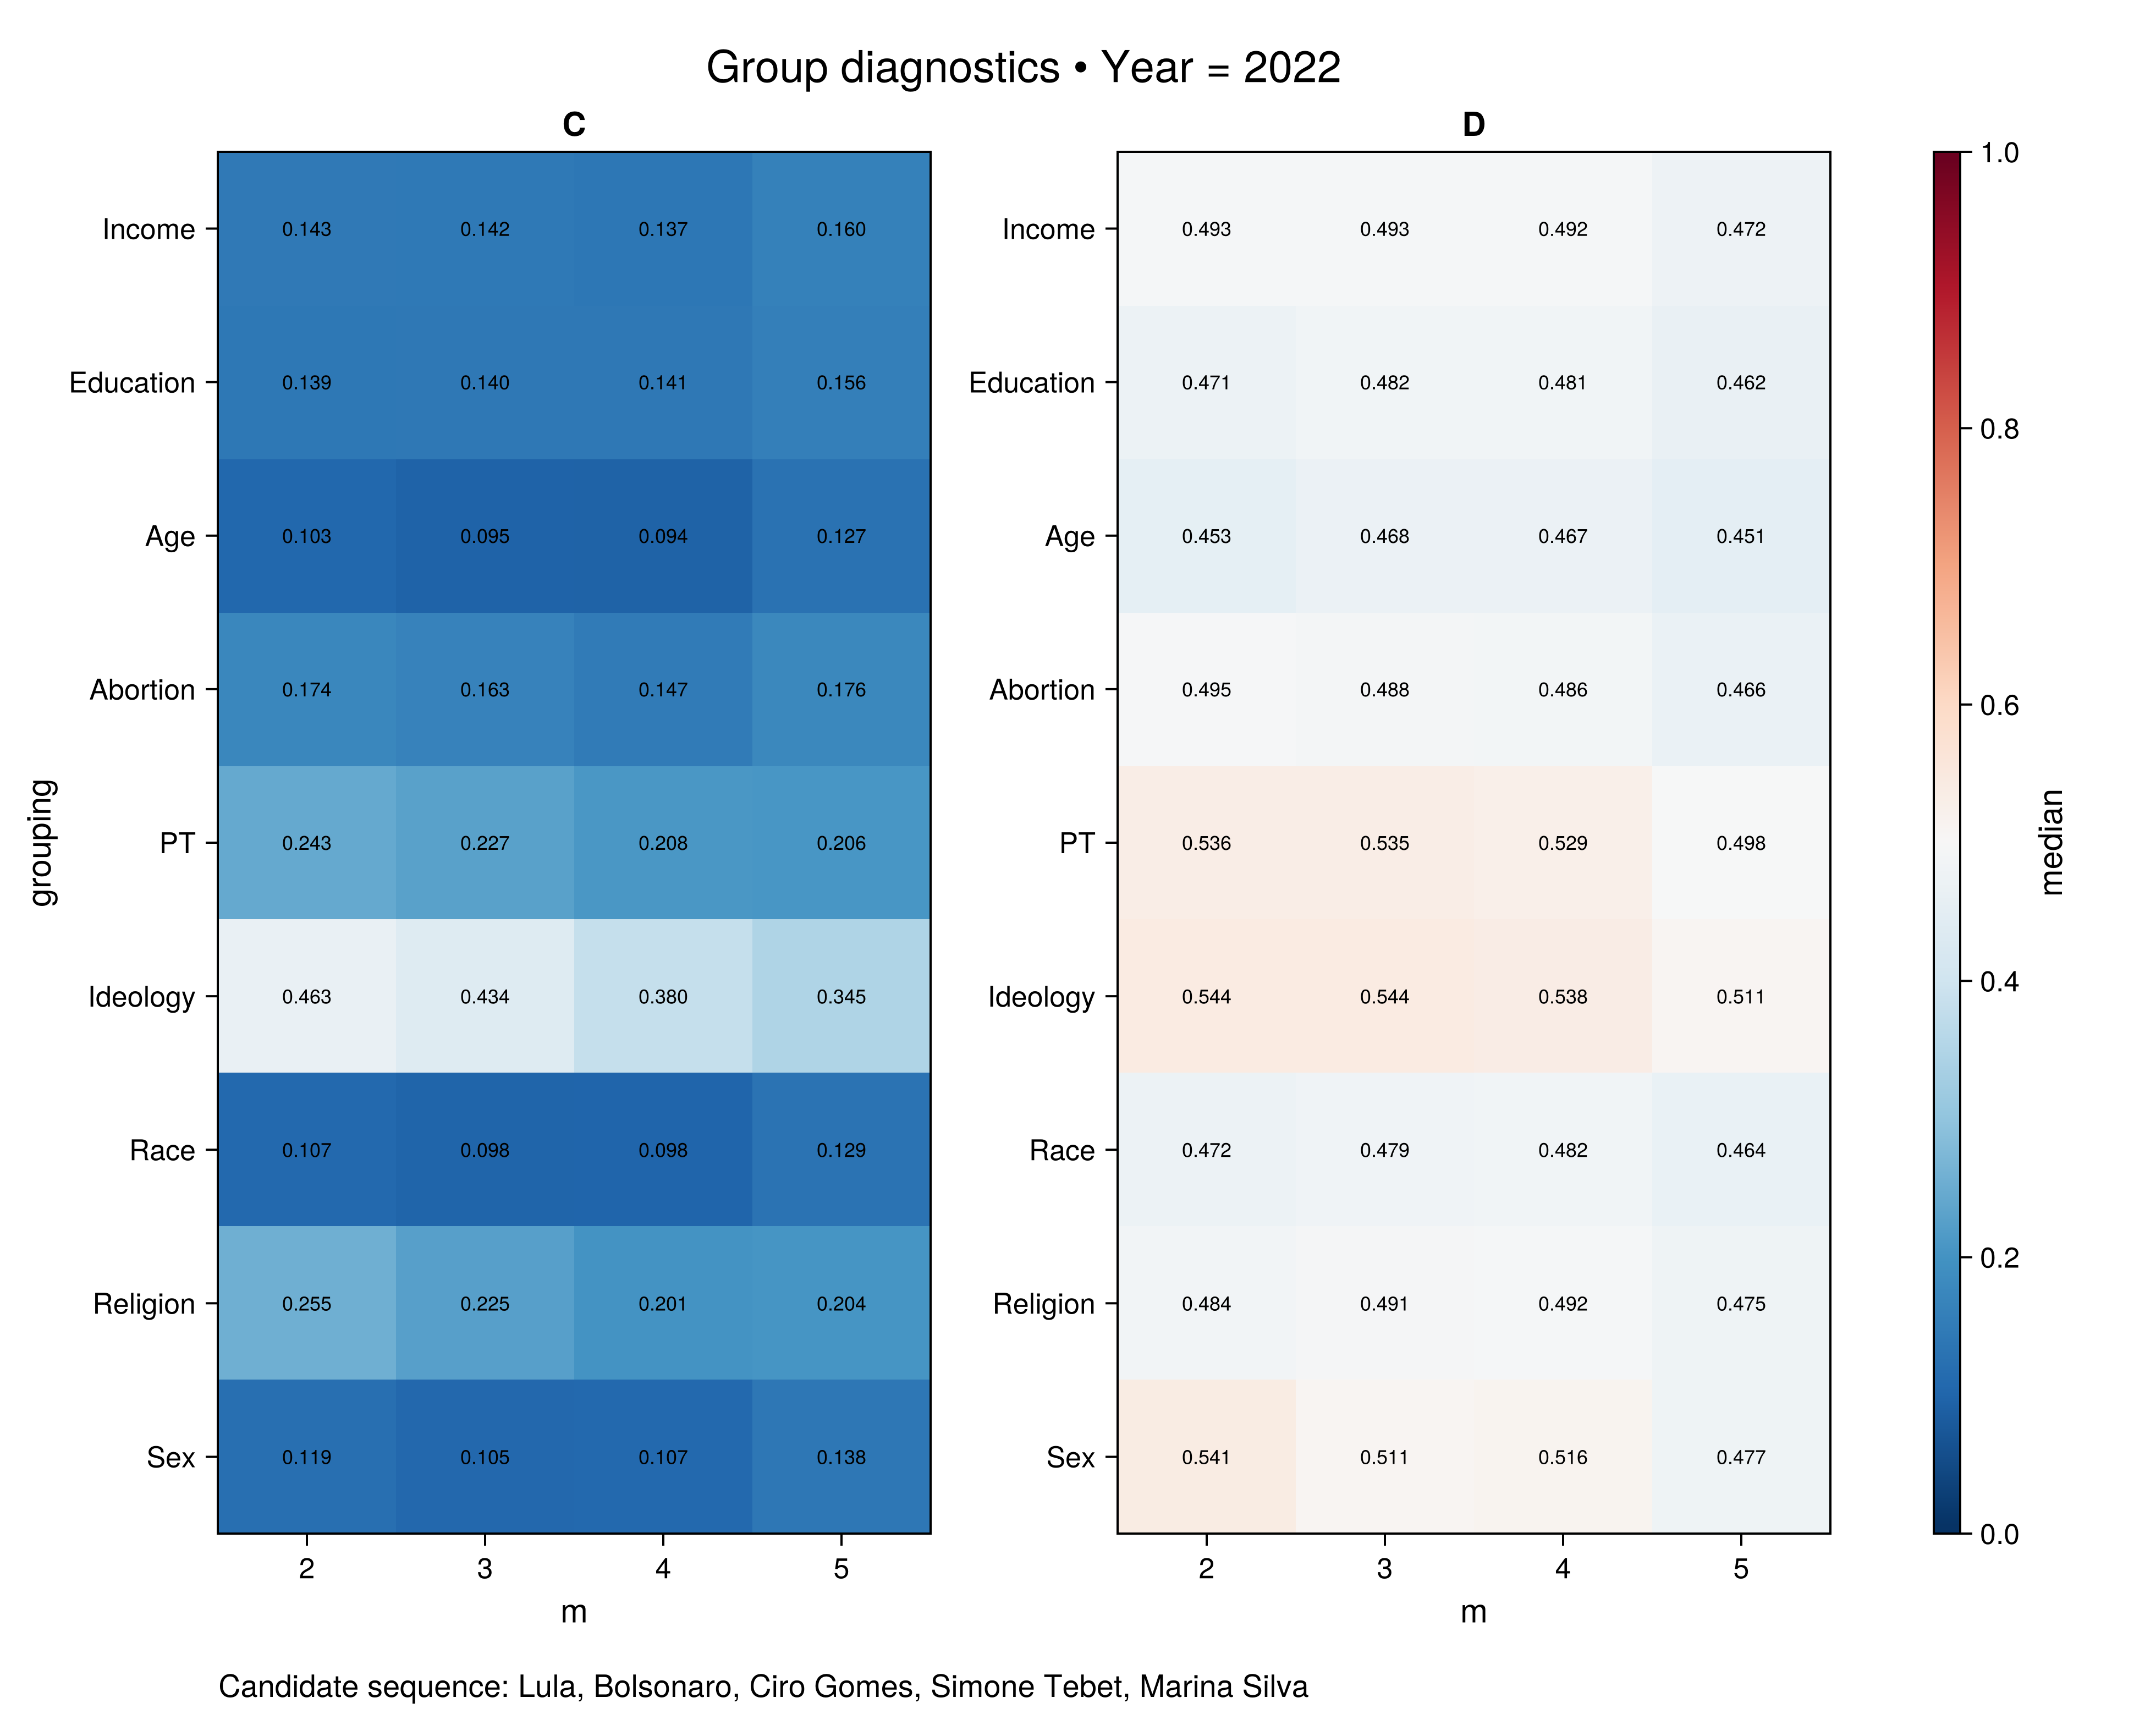
\includegraphics[width=\textwidth,keepaspectratio]{imgs/2022_group_C_D.png}
  \caption{Group diagnostics in 2022: within-group coherence \(C\) and between-group divergence \(D\).}
  \label{fig:group-2022}
\end{figure}

In 2022, the group-based measures show a clearer structure than in the
previous waves, but not because all groupings become equally informative.
Race, age, education, income, and sex remain weak discriminators. Their
within-group coherence \(C\) is low and their between-group divergence \(D\) is
moderate, so they do not define compact and externally differentiated
preference blocs.

Abortion, religion, and PT evaluation are more informative than the purely
demographic partitions. Religion has relatively high divergence, but its
coherence remains below the main political variables. PT evaluation is
stronger: its \(D\) remains high across candidate-set sizes, indicating that
PT-defined groups have distinct fitted consensuses. However, its within-group
coherence is only moderate to low. Thus, PT evaluation still distinguishes
group consensuses, but its within-group coherence is not high enough for it to
be the most informative partition in 2022.

This marks a change from 2006. In 2006, PT evaluation was the main political
grouping, especially in the binary comparison. By 2022, PT remains relevant,
but its structuring role is weaker because the coherence component is lower.
The decline is not driven primarily by a disappearance of between-group
divergence: PT-defined groups remain far apart in consensus space. The more
important change is that respondents within the same PT category are less
internally coherent. In group-structuration terms, PT still differentiates
groups externally, but it no longer produces the most internally organized
subprofiles.

Ideology is the clear outlier in 2022. It has the highest within-group
coherence \(C\) and the highest or near-highest between-group divergence \(D\)
across candidate-set sizes. Its values also decline as more alternatives are
added, which is expected: larger candidate sets make rankings harder to
compress into internally coherent group consensuses. But even after this
decline, ideology remains above the other partitions on the relevant
diagnostics. Unlike PT, ideology combines internal coherence with external
divergence. The 2022 group analysis therefore identifies ideology as the most
informative partition among those examined, followed by PT evaluation, while
demographic partitions remain weak.

The aggregate contrast with 2006 is that the system becomes more externally
divergent without becoming uniformly more internally cohesive. For most
groupings, \(D\) is higher in 2022 than in 2006, while \(C\) is lower or only
modestly positive. This means that group consensuses are farther apart, but
group members are not necessarily more tightly clustered around those
consensuses. Ideology in 2022 is the main exception: it is associated both with
relatively high internal coherence and with distant group consensuses.

Taken together, the global and group-based measures support a more precise
interpretation than a simple increase in polarization. The profile becomes
more structured over time, but it does not bifurcate into two internally
homogeneous and mutually opposed blocs. The global measures show that pairwise
antagonism increases from 2006 to 2022. \(\Psi\) is already moderate to high
in 2006, rises in 2018, and reaches its highest values in 2022, where it
remains high even after the candidate set expands beyond the binary
Lula--Bolsonaro comparison. Thus, the temporal change is not the emergence of
antagonism from a neutral baseline. It is an intensification of dissent from
an already nontrivial level.

The reversal-based measures clarify the structure of this intensification.
At \(m=2\), the binary comparison mechanically forces all opposition into a
single reversal field. This is why \(\Psi=R\), \(\kappa=1\), and
\(ENRP=1\). Once \(m\geq 3\), the structure becomes identifiable: reversal
mass can be distributed across multiple opposed rankings. In all three waves,
\(RHHI\) falls relative to the binary case, and \(ENRP>1\), showing that
antagonism does not collapse onto a single divide. But the decline is not the
same across years. In 2022, \(R\) remains high even for larger candidate sets,
\(RHHI\) remains above the earlier waves at comparable values of \(m\), and
the effective number of reversal pairs is lower. With four alternatives, for
example, the effective number of reversal pairs declines from roughly \(5.6\)
in 2006 to \(4.2\) in 2018 and \(3.0\) in 2022; with five alternatives, it
declines from \(18.65\) to \(13.43\) and then to \(7.72\). Hence the process
is not only one of increasing antagonism. It is also one of increasing
compression: more reversal mass is carried by fewer effective regions of the
ranking space.

The group-based measures compare how much of this organization is visible
under the partitions examined. In 2006, PT evaluation is the only grouping
that clearly stands above the demographic partitions. It has higher coherence,
divergence, especially in the binary comparison. But this structure weakens as
additional alternatives are admitted.
In 2018, the missingness of PT evaluation prevents using it directly, and the
relevant political grouping is instead respondents' score for Lula. Lula score
is the clearest grouping in that year: it is the only 2018 partition that
combines high within-group coherence with high between-group divergence.
Ideology is also informative, but it remains below Lula score.

By 2022, the ranking of informative groupings changes again. PT evaluation
remains informative, but it no longer produces the most internally coherent
subprofiles. Its between-group divergence remains high, which means that
PT-defined consensuses are still far apart, but its coherence is lower. In
2022, ideology is the clear outlier. It has the highest coherence and the
highest or near-highest divergence across candidate-set sizes. The resulting sequence is therefore not
simply PT versus anti-PT throughout the period. Among the groupings examined,
the most informative partition is PT evaluation in 2006, Lula score in 2018,
and ideology in 2022.

This matters for the interpretation of the usual ``two Brazils'' narrative.
Binary electoral margins can invite the interpretation that a close race is
itself evidence of polarization, because with \(m=2\) the measures collapse to
the normalized pair margin and all reversal is forced into one field. But the
multiparty profile shows something different. The observed preference profiles
are not well described as two impermeable camps with internally unanimous
preferences. The evidence points instead to structuration without bifurcation.
Dissent becomes stronger, exact reversal mass becomes larger, and the occupied
ranking space becomes more compressed, especially in 2022. Yet opposition
remains distributed across multiple rankings and multiple reversal fields.

The most accurate summary is therefore not that Brazil simply became
polarized, but that the observed preference profiles became more organized.
This organization is visible globally as higher pairwise antagonism, higher
reversal mass, and greater concentration of reversal fields. At the group
level, PT evaluation and Lula score matter a great deal in the observed
profiles: PT evaluation is the most informative grouping in 2006, and Lula
score is the most informative grouping in 2018. The striking change is that,
in 2022, ideology is the strongest group-level organizer among the partitions
examined, surpassing PT evaluation across the main measures. This does not
make PT or Lula irrelevant to the analysis. Rather, it shows that the strongest
observed political grouping changes across waves: from PT evaluation, to Lula
score, to ideological self-placement. The observed preference profiles are
therefore neither random fragmentation nor pure binary polarization. They form
a structured multiparty configuration of multiple oppositions, increasingly
compressed around ideological distinctions in 2022.

\section*{Conclusion}

In this article, I extend the study of ``polarization'' to settings with more than
two evaluated objects by focusing on relative evaluations, or preferences, and
using the ordinal information contained in survey responses. I develop global
and group-based measures of preference-profile structuration and apply them to
Brazilian presidential evaluations in 2006, 2018, and 2022. The global measures
show increasing antagonism and organization over time, but the magnitude and
interpretation of this increase depend on the number of alternatives considered
and on whether one measures pairwise opposition, exact reversal mass, or the
concentration of reversal fields. Taken together, the results point to
structuration without bifurcation: disagreement becomes stronger and more
compressed, but it does not collapse into two internally unanimous and mutually
antagonistic camps. The group-based diagnostics show that, among the groupings
examined here, the most informative political partition changes across waves:
PT evaluation in 2006, Lula score in 2018, and self-identified ideology in
2022. By contrast, most demographic partitions tested here, such as race, sex,
age, education, and income, remain weakly informative.

In the context of preferences over candidates, this work drastically qualifies
the hegemonic narrative of a divided country and points toward a more fruitful
research agenda centered on the dynamic structuring of preference profiles \parencite{
  feld1990collectivities}. More radically, although ordinal information implies a universe of
profiles that is formally distinct than that defined by a cardinal interval, the
analysis of evaluative social conflicts would be enriched by a pullback to the
space of reasons underlying relative evaluations. In a context of elite
radicalization, it is relevant to probe the motivational content of citizens’
preferences over candidates, instead of just tallying ``affect''. That is: what
is the form taken by the reasons, or rationalizations, offered for such
evaluations? 

% Although it lies outside the direct analytical scope of this article, the
% results presented here have broader implications. I have shown that the
% polarization discourse may be well suited to majoritarian contexts with
% \(ENP=2\), since the measures agree, but travels poorly to settings like Brazil.
% This is a logical/structural constraint: once \(m>2\), the object is
% qualitatively distinct, a recurrent theme in politics
% \parencite{black1998theory}. A hypothesis for future research is that
% majoritarian institutions, via Duvergerian pressures toward two-party
% competition, can induce informational bottlenecks that render preference
% structure legible primarily as binary opposition. Testing this requires
% comparative designs across electoral systems.

% Its misalignment with multiparty systems also has normative implications. The
% polarization discourse has a well-defined nationality and partisan identity and
% is often deployed as a political-communication frame associated with ‘culture
% war’ rhetoric \parencite{fiorina08_polit_polar_americ_public,
%   schedler23_rethin_polit_polar, dimaggio2003myth, sen2007identity}. Social
% phenomena do not impose themselves on perception; they require (re)construction
% through cognitive artifacts—surveys, theories, measures—that render a nebulous
% reality intelligible \parencite{ostrom1990problems, dos1990discurso}. These
% artifacts are not neutral: they belong to the discursive sphere that delimits
% the possibility space for sociopolitical action \parencite{orr2018entanglement}.
% Within this broader context, this work participates in the responsible
% construction of such instruments of representation, a core functional task of the
% political-science community.


% grafico de evolucao do PT

% grafico da evoluacao da ideologia


% Apendice: Grafico da medida global comparando imputacoes nos tres anos.




% Sejam \(p_1\) o perfil com os cinco políticos mais conhecidos e \(p_2\) o perfil com todos os políticos. Os resultados são:

% \begin{align}
%   \Psi(p_1) &= 0{,}90 \\
%   R(p_1) &= 0{,}67, \quad \kappa(\text{op}(p_1)) = 0{,}02 \Rightarrow RHHI(p_1) \approx 0{,}12
% \end{align}

% Para \( p_2 \):

% \begin{align}
%   \Psi(p_2) &= 0{,}84 \\
%   R(p_2) &= 0{,}00 \Rightarrow RHHI(p_2) = 0
% \end{align}

\printbibliography

\appendix

\section{Mathematical Appendix}
\subsection{Relationship Between \(C\) and \(D\)}
\label{app:c-d-relationship}

This appendix states the relationship between within-group coherence \(C\) and
the member-to-other-consensus divergence statistic \(D\). The key point is that
\(D\) is not only a distance between group consensuses. Because it averages the
distance from individual rankings in one group to the consensus rankings of
other groups, it partly reflects the internal dispersion of the group being
evaluated.

Let \(A\) be the active candidate set, with \(|A|=m\), and let
\(\mathcal{L}(A)\) denote the set of linear orders over \(A\). For each group
\(G_g\) of size \(n_g\), define the normalized average Kendall loss of a
candidate consensus ranking \(\rho \in \mathcal{L}(A)\) as
\[
\ell_g(\rho)
=
\frac{1}{n_g}
\sum_{x \in G_g}
\frac{d_\tau(x,\rho)}{\binom{m}{2}},
\]
where \(x\) is the observed ranking of an individual member of \(G_g\), and
\(d_\tau\) is Kendall tau distance.

The consensus set of group \(g\) is the set of rankings that minimize this loss:
\[
M_g
=
\arg\min_{\rho \in \mathcal{L}(A)} \ell_g(\rho).
\]
When \(M_g\) is not a singleton, consensus-dependent quantities are averaged
over the minimizing rankings. Let \(\bar{\ell}_g(M_h)\) denote the average loss
of group \(g\)'s members relative to the consensus set of group \(h\):
\[
\bar{\ell}_g(M_h)
=
\frac{1}{|M_h|}
\sum_{\rho \in M_h}
\ell_g(\rho).
\]

Define the within-group dispersion of \(G_g\) around its own consensus set as
\[
W_g
=
\bar{\ell}_g(M_g)
=
\min_{\rho \in \mathcal{L}(A)} \ell_g(\rho).
\]
The raw coherence of group \(g\) is
\[
C_g^\star
=
1-W_g.
\]
Aggregating by group size gives
\[
C^\star
=
\sum_{g=1}^{k}
\frac{n_g}{n}C_g^\star,
\qquad
n=\sum_{g=1}^{k}n_g.
\]
Therefore the aggregate within-group dispersion is
\[
W
=
\sum_{g=1}^{k}
\frac{n_g}{n}W_g
=
1-C^\star.
\]

The raw coherence statistic \(C^\star\) is not bounded below by \(0\), but by
\(1/2\). To see this, fix any ranking \(\rho \in \mathcal{L}(A)\), and let
\(\rho^{\mathrm{rev}}\) be its reverse. For any individual ranking \(x\),
\[
d_\tau(x,\rho)
+
d_\tau(x,\rho^{\mathrm{rev}})
=
\binom{m}{2}.
\]
After normalizing and averaging over members of group \(g\), this implies
\[
\ell_g(\rho)
+
\ell_g(\rho^{\mathrm{rev}})
=
1.
\]
Hence at least one of \(\rho\) or \(\rho^{\mathrm{rev}}\) has average normalized
loss no greater than \(1/2\). Since \(W_g\) is the minimum of \(\ell_g(\rho)\)
over all rankings,
\[
W_g \le \frac{1}{2}.
\]
It follows that \(C_g^\star \ge 1/2\), and therefore \(C^\star \ge 1/2\). This
motivates the rebased coherence statistic
\[
C
=
2C^\star-1,
\]
which places the no-structure baseline at zero.

The group divergence statistic is defined as the average distance from members
of one group to the consensus set of other groups:
\[
D
=
\frac{1}{k-1}
\sum_{g=1}^{k}
\sum_{h\neq g}
\frac{n_g}{n}
\bar{\ell}_g(M_h).
\]
For each ordered pair of distinct groups \((g,h)\), add and subtract group
\(g\)'s own internal dispersion \(W_g\):
\[
\bar{\ell}_g(M_h)
=
W_g
+
\left[
\bar{\ell}_g(M_h)-W_g
\right].
\]
Substituting into the definition of \(D\) yields
\[
D
=
\frac{1}{k-1}
\sum_{g=1}^{k}
\sum_{h\neq g}
\frac{n_g}{n}W_g
+
\frac{1}{k-1}
\sum_{g=1}^{k}
\sum_{h\neq g}
\frac{n_g}{n}
\left[
\bar{\ell}_g(M_h)-W_g
\right].
\]
The first term simplifies because \(W_g\) depends only on \(g\), not on \(h\):
\[
\frac{1}{k-1}
\sum_{g=1}^{k}
\sum_{h\neq g}
\frac{n_g}{n}W_g
=
\sum_{g=1}^{k}
\frac{n_g}{n}W_g
=
W.
\]
The bracketed term is nonnegative because \(W_g\) is the minimum possible value
of \(\ell_g(\rho)\) over rankings \(\rho\), and every member of \(M_h\) is a
ranking in \(\mathcal{L}(A)\). Hence the second term is a nonnegative quantity,
and
\[
D \geq W.
\]
Since \(W=1-C^\star\),
\[
D \geq 1-C^\star.
\]
Using the rebased statistic \(C=2C^\star-1\), this is equivalently
\[
D \geq \frac{1-C}{2}.
\]
This relationship is the reason \(C\) and \(D\) are reported separately in the
main analysis. A high value of \(D\) can reflect external divergence between
group consensuses, internal dispersion within the group being evaluated, or
both.

\subsection{Reference Profiles and Diagnostic Behavior}
\label{app:measures-action}


This appendix reports the behavior of the diagnostics on a set of paradigmatic
profiles. The point of these cases is not empirical realism, but interpretation:
they show why pairwise antagonism, exact reversal mass, reversal concentration,
and group structuration are distinct objects.

\subsubsection{Benchmark profiles}

Let \(A\) be a finite set of \(m\) alternatives, and let \(L(A)\) be the set of
linear orders over \(A\). For a ranking \(r \in L(A)\), let \(-r\) denote its
reversal. Consider the following generating functions:
\begin{itemize}
  \item \(u\): generates a profile in which all individuals share the same
  ordering over \(m\) alternatives. It is represented by the proportion map
  \[
    \{r_{\star}:1\}.
  \]
  \footnote{\(u\) for \textbf{u}nanimity.}

  \item \(e\): generates a profile in which all \(m!\) orderings appear with
  equal frequency. It is represented by
  \[
    \{r_1:\tfrac{1}{m!},\ldots,r_{m!}:\tfrac{1}{m!}\}.
  \]
  \footnote{\(e\) for \textbf{e}quiprobable.}

  \item \(i\): generates a profile in which half the individuals have an
  ordering \(r_{\star}\) and the other half have its reversal \(-r_{\star}\).
  It is represented by
  \[
    \{r_{\star}:\tfrac{1}{2},-r_{\star}:\tfrac{1}{2}\}.
  \]
  \footnote{\(i\) for \textbf{i}nversion.}
\end{itemize}

For any number of alternatives \(m \geq 2\), these profiles satisfy:
\begin{align}
  \Psi(i(m)) &= \Psi(e(m)) = R(i(m)) = R(e(m)) = RHHI(i(m)) = 1, \\
  \Psi(u(m)) &= R(u(m)) = RHHI(u(m)) = 0.
\end{align}

The intuition is straightforward. In the unanimous profile \(u(m)\), every
individual ranks every pair of alternatives in the same direction. Hence there
is no pairwise antagonism and no exact reversal mass. In the inversion profile
\(i(m)\), every pairwise comparison is split evenly, and all profile mass lies
on one ranking and its reversal. Thus pairwise antagonism, exact reversal mass,
and reversal concentration are all maximal.

The equiprobable profile \(e(m)\) is different. It also maximizes pairwise
antagonism and exact reversal mass, but the reversal mass is spread across all
possible reversal fields. This is why \(RHHI\) depends on the number of
alternatives in equiprobable profiles.

For the profile \(e(m)\), each of the \(m!\) possible orderings occurs with
frequency \(1/m!\). Consider a pair of reversal orderings \((r,-r)\). Since
both have the same frequency, the local reversal component is
\[
  \operatorname{op}(r)
  =
  2\min\left\{\frac{1}{m!},\frac{1}{m!}\right\}
  =
  \frac{2}{m!}.
\]
There are \(m!/2\) such reversal pairs. Therefore,
\[
  R(e(m))
  =
  \frac{m!}{2}\cdot \frac{2}{m!}
  =
  1.
\]
Since \(R(e(m))=1\), each reversal field has normalized reversal share
\[
  q_i = \frac{2}{m!}.
\]
Applying the Herfindahl--Hirschman index to
\(\mathbf q=(q_1,\ldots,q_{m!/2})\), we obtain
\[
  \kappa(q(e(m)))
  =
  \frac{m!}{2}
  \left(\frac{2}{m!}\right)^2
  =
  \frac{2}{m!}.
\]
Finally, since \(RHHI\) is the geometric mean between reversal intensity \(R\)
and reversal concentration \(\kappa\),
\[
  RHHI(e(m))
  =
  \sqrt{R(e(m))\kappa(q(e(m)))}
  =
  \sqrt{\frac{2}{m!}}.
\]

For example:
\begin{align}
  R(e(3)) &= 1,
  &
  \kappa(q(e(3))) &= \frac{1}{3},
  &
  RHHI(e(3)) &\approx 0.577, \\
  R(e(4)) &= 1,
  &
  \kappa(q(e(4))) &= \frac{1}{12},
  &
  RHHI(e(4)) &\approx 0.289.
\end{align}
More generally, as \(m\) grows,
\[
  RHHI(e(m)) = \sqrt{\frac{2}{m!}} \to 0.
\]
Thus, \(RHHI\) approaches zero in equiprobable profiles not because pairwise
antagonism disappears, nor because exact reversal mass disappears, but because
that reversal mass becomes maximally diffuse across the ranking space.

By recalling that \(1/\kappa\) gives the effective number of reversal pairs,
we have for \(e(m)\):
\[
  ENRP(e(m))
  =
  \frac{1}{\kappa(q(e(m)))}
  =
  \frac{m!}{2}.
\]
This is the maximum possible value. Thus, \(e(m)\) profiles correspond to
maximal dispersion, or minimal concentration, in the reversal component.

In this way, \(RHHI\) distinguishes between the profiles \(i(m)\) and \(e(m)\).
Both maximize \(\Psi\), and both maximize \(R\). However, \(i(m)\) concentrates
all reversal mass in one reversal field, whereas \(e(m)\) distributes reversal
mass across the maximum possible number of reversal fields. Equivalently,
\(ENRP\) ranges from \(1\) in the pure inversion profile to \(m!/2\) in the
equiprobable profile.

\subsubsection{Group diagnostics}

Regarding the behavior of the group diagnostics \(C\) and \(D\), it is useful
to interpret them against two reference profiles.

First, consider an \(e\)-profile where every possible ranking appears with
equal frequency within each group. In this case, group labels do not organize
the profile. The best consensus ranking still mismatches group members on
about half of all pairwise comparisons, so \(C^{\star}\approx 1/2\) and the
rebased coherence is \(C\approx 0\). The divergence statistic \(D\), however,
need not be close to zero, because it compares group members to other groups'
fitted consensuses. In an unstructured ranking space, these consensuses are
still typically at nonzero Kendall distance from individual rankings. This is
why \(D\) must be interpreted together with \(C\): low \(C\) indicates that a
large part of the distance in \(D\) can come from internal dispersion rather
than from compact group structuration.

Second, consider a unanimous profile \(u(m)\), where all respondents share the
same ranking. Then internal coherence is maximal, so \(C=1\). If all groups
share that same ranking, their consensuses coincide and \(D=0\): there is no
group divergence because there is no disagreement to organize.

By contrast, if each group is internally unanimous but different groups hold
different, possibly opposed, rankings, then \(C=1\) and \(D\) is high. These
reference cases show why the diagnostics should not be collapsed into a single
score. \(C\) captures internal consolidation, while \(D\) captures distance to
external consensuses.




\subsection{Derivations for m=2}
\label{sec:appendixB}
For \(\kappa = 1\) when \(m=2\) note that the number of possible rankings is \(2! = 2\). The set of rankings is \(\{ A \succ B,\; B \succ A \}\), and there is only one possible reversed pair: \((A \succ B,\; B \succ A)\). Let \(p\) and \(1-p\) be the proportions of voters with each ranking. Then, the local reversal component is \(r = 2 \cdot \min(p, 1 - p)\). Since there is only this pair, the total reversal is just \(r\). Thus, the normalized distribution has \(q_1 = r/R = 1\), which implies \(\kappa = \sum_i q_i^2 = 1^2 = 1\).

Now, for \(m=2\) alternatives, \(\Psi\) and \(R\) coincide. Let there be \(m=2\) alternatives, \(A\) and \(B\), and \(n\) voters. Denote
\[
n_{AB}=\#\{i: A\succ_i B\},\qquad n_{BA}=n-n_{AB}.
\]
By \textcite{can2015measuring}, for \(m=2\) there is only one unordered pair \(\{A,B\}\), so
\[
\Psi(p)
= \frac{n - d_{AB}(p)}{n \binom{2}{2}}
= \frac{n - d_{AB}(p)}{n},
\]
where
\[
d_{AB}(p) = \big|n_{AB}-n_{BA}\big|
= \big|n_{AB} - (n-n_{AB})\big|
= \big| 2n_{AB} - n \big|.
\]
Hence
\[
\Psi(p) = 1 - \frac{|2n_{AB} - n|}{n}.
\]
There are only two linear orders, \(AB\) and \(BA\), which are reversals. Let the proportions be
\[
p(AB) = \frac{n_{AB}}{n}, \qquad p(BA) = \frac{n_{BA}}{n}.
\]
By definition,
\[
R(p) = 2\min\{p(AB), p(BA)\}
= \frac{2}{n} \min\{n_{AB},\, n - n_{AB}\}.
\]
Using \(\min\{x,y\} = \frac{x+y - |x-y|}{2}\) with \(x=n_{AB}\), \(y=n-n_{AB}\), we obtain
\[
\min\{n_{AB}, n-n_{AB}\}
= \frac{n - |n - 2n_{AB}|}{2},
\]
and
\[
R(p) = \frac{2}{n} \cdot \frac{n - |n - 2n_{AB}|}{2}
= 1 - \frac{|n - 2n_{AB}|}{n}
= 1 - \frac{|2n_{AB} - n|}{n}.
\]
Thus, we have \(\Psi(p) = R(p)\) for \(m=2\).


\section{Methodological Appendix}
\subsection{Pattern-conditional linearization with Jeffreys smoothing}
\label{app:pattern-linearization}

The survey records evaluations as ratings rather than complete strict rankings.
For a respondent \(i\), let \(A_m\) denote the candidate set and let
\(x_i(a)\) be the imputed rating assigned to candidate \(a\in A_m\). These
ratings induce a weak order \(w_i\) over \(A_m\). Equivalently, \(A_m\) is
partitioned into indifference classes
\[
B_{i1},B_{i2},\ldots,B_{iK_i},
\]
where all candidates in the same class receive the same rating and the classes
are ordered from higher to lower rating:
\[
x_i(a) > x_i(b)
\quad\text{whenever}\quad
a\in B_{ik},\ b\in B_{i\ell},\ k<\ell .
\]
Linearization preserves this between-class ordering and resolves only
within-class indifferences.

Let \(\mathcal E(w)\) be the set of all strict linear extensions compatible
with weak order \(w\). Thus,
\[
\mathcal E(w)
=
\{\pi\in \mathcal L(A_m): \pi \text{ preserves the strict comparisons in } w\},
\]
where \(\mathcal L(A_m)\) is the set of all \(m!\) linear orders over \(A_m\).
If the weak order has indifference classes \(B_1,\ldots,B_K\), then
\[
|\mathcal E(w)|=\prod_{k=1}^K |B_k|!.
\]
The random-tie linearizer samples uniformly from \(\mathcal E(w)\):
\[
p_{\mathrm{unif}}(\pi\mid w)
=
\frac{1}{|\mathcal E(w)|},
\qquad
\pi\in\mathcal E(w).
\]

The pattern-conditional linearizer instead estimates a conditional distribution
over compatible refinements. Let \(n_w(\pi)\) denote the number of observed
cases in the relevant empirical stratum with weak-order pattern \(w\) whose
strict refinement is \(\pi\in\mathcal E(w)\). The raw empirical estimator would
be
\[
\widehat p(\pi\mid w)
=
\frac{n_w(\pi)}
{\sum_{\pi'\in\mathcal E(w)}n_w(\pi')}.
\]
This estimator is undesirable in sparse strata because it assigns probability
zero to unobserved refinements and probability one to a refinement observed only
once when no alternatives have been observed.

I therefore use Jeffreys smoothing. For each compatible refinement
\(\pi\in\mathcal E(w)\), define
\[
\widetilde p_\alpha(\pi\mid w)
=
\frac{n_w(\pi)+\alpha}
{\sum_{\pi'\in\mathcal E(w)}\{n_w(\pi')+\alpha\}},
\qquad
\alpha=\frac12.
\]
Equivalently, if
\[
N_w=\sum_{\pi'\in\mathcal E(w)} n_w(\pi'),
\]
then
\[
\widetilde p_{1/2}(\pi\mid w)
=
\frac{n_w(\pi)+1/2}
{N_w+\frac12|\mathcal E(w)|}.
\]
This is the posterior mean under a symmetric Dirichlet prior with parameter
\(\alpha=1/2\) over the vector of refinement probabilities. It is symmetric
across refinements, prevents degenerate zero and one probabilities in sparse
cells, and regularizes less strongly than Laplace smoothing
\((\alpha=1)\).

The behavior of the estimator is straightforward. If no empirical refinements
are observed for a weak-order pattern, \(N_w=0\), then
\[
\widetilde p_{1/2}(\pi\mid w)
=
\frac{1}{|\mathcal E(w)|},
\]
so the procedure reduces to uniform tie-breaking. If \(N_w\) is large, the
pseudo-counts become negligible and
\[
\widetilde p_{1/2}(\pi\mid w)
\approx
\widehat p(\pi\mid w).
\]
Thus the rule interpolates between uniform tie-breaking in empty or very sparse
strata and empirical pattern-conditional tie-breaking in well-populated strata.

The linearization step for respondent \(i\) is therefore:
\[
\pi_i \sim \widetilde p_{1/2}(\cdot\mid w_i),
\qquad
\pi_i\in\mathcal E(w_i).
\]
This preserves the ordinal information contained in the ratings while allowing
recurrent empirical refinements of ties to inform the completed ranking. The
purpose is not to recover a latent ``true'' strict order behind every tie, but
to avoid injecting purely uniform noise when the data contain stable
tie-breaking structure.

\subsection{Nested variance decomposition}
\label{app:nested-variance-decomposition}

For a fixed analysis cell, defined by wave, scenario, candidate-set size
\(m\), measure, grouping, and pipeline specification, let
\[
Y_{brk}
\]
denote the value of the measure computed from bootstrap replicate
\(b\in\{1,\ldots,B\}\), imputation replicate \(r\in\{1,\ldots,R\}\), and
linearization replicate \(k\in\{1,\ldots,K\}\). The indices are nested:
linearization varies within imputed datasets, imputation varies within
bootstrap pseudo-profiles, and bootstrap resampling varies over pseudo-profiles.

Define the lower-level conditional means
\[
\bar Y_{br\cdot}
=
\frac{1}{K}\sum_{k=1}^K Y_{brk},
\]
and
\[
\bar Y_{b\cdot\cdot}
=
\frac{1}{R}\sum_{r=1}^R \bar Y_{br\cdot}.
\]
The overall mean for the fixed analysis cell is
\[
\bar Y_{\cdot\cdot\cdot}
=
\frac{1}{B}\sum_{b=1}^B \bar Y_{b\cdot\cdot}.
\]

The bootstrap component is the variance across bootstrap-level conditional
means:
\[
V_{\mathrm{boot}}
=
\operatorname{Var}_b(\bar Y_{b\cdot\cdot}).
\]
This term captures variation induced by changing the weighted pseudo-profile
while averaging over the imputation and linearization replicates nested within
that pseudo-profile.

The imputation component is the average, over bootstrap replicates, of the
within-bootstrap variance across imputation-level conditional means:
\[
V_{\mathrm{imp}}
=
\frac{1}{B}\sum_{b=1}^B
\operatorname{Var}_r(\bar Y_{br\cdot}).
\]
This term captures variation induced by different imputations of the same
bootstrap pseudo-profile, after averaging over the linearization replicates
nested within each imputed dataset.

The linearization component is the average, over bootstrap and imputation
replicates, of the within-\((b,r)\) variance across linearizations:
\[
V_{\mathrm{lin}}
=
\frac{1}{BR}
\sum_{b=1}^B\sum_{r=1}^R
\operatorname{Var}_k(Y_{brk}).
\]
This term captures variation induced by completing weak preferences into
linear orders conditional on a fixed bootstrap pseudo-profile and a fixed
imputed dataset.

The reported total is the sum of these nested components:
\[
V_{\mathrm{tot}}
=
V_{\mathrm{boot}}
+
V_{\mathrm{imp}}
+
V_{\mathrm{lin}}.
\]
With the balanced-tree and population-variance convention used in the
replication code, this total equals the empirical variance of the leaf-level
values:
\[
V_{\mathrm{tot}}
=
\operatorname{Var}_{b,r,k}(Y_{brk}).
\]
The point of the decomposition is therefore not to define a different total
variance. It is to partition the empirical simulation variance according to the
nested stochastic operations that generated it. Variation across \(k\) is
interpreted as linearization variability only after conditioning on \(b\) and
\(r\); variation across \(r\) is interpreted as imputation variability only
after conditioning on \(b\); and variation across \(b\) is interpreted as
bootstrap variability only after averaging over the lower-level stochastic
operations.

Explicitly, the implementation uses the population-variance convention
\[
\operatorname{Var}_b(\bar Y_{b\cdot\cdot})
=
\frac{1}{B}
\sum_{b=1}^B
\left(
\bar Y_{b\cdot\cdot}
-
\bar Y_{\cdot\cdot\cdot}
\right)^2,
\]
with analogous formulas for \(\operatorname{Var}_r\) and
\(\operatorname{Var}_k\). Under this convention, a component with only one
realized branch is set to zero. Thus, if \(B=1\), the bootstrap component is
zero; if \(R=1\), the imputation component is zero; and if \(K=1\), the
linearization component is zero.

The decomposition is computed within fixed analysis cells. In particular,
candidate-set size \(m\) is part of the conditioning information, not a
stochastic source of variation. This is important because changing \(m\) changes
the ranking space, the number of possible linear orders, the sparsity of the
profile, and the scale on which several measures vary. Comparisons across
pipeline specifications are therefore made within the same wave, scenario,
candidate-set size \(m\), measure, and grouping. Summaries that pool over
multiple values of \(m\) are used only as compact descriptive diagnostics across
analysis cells, not as the primary variance decomposition.


\begin{figure}[htp]
  \centering
  \vspace{-1.2cm}
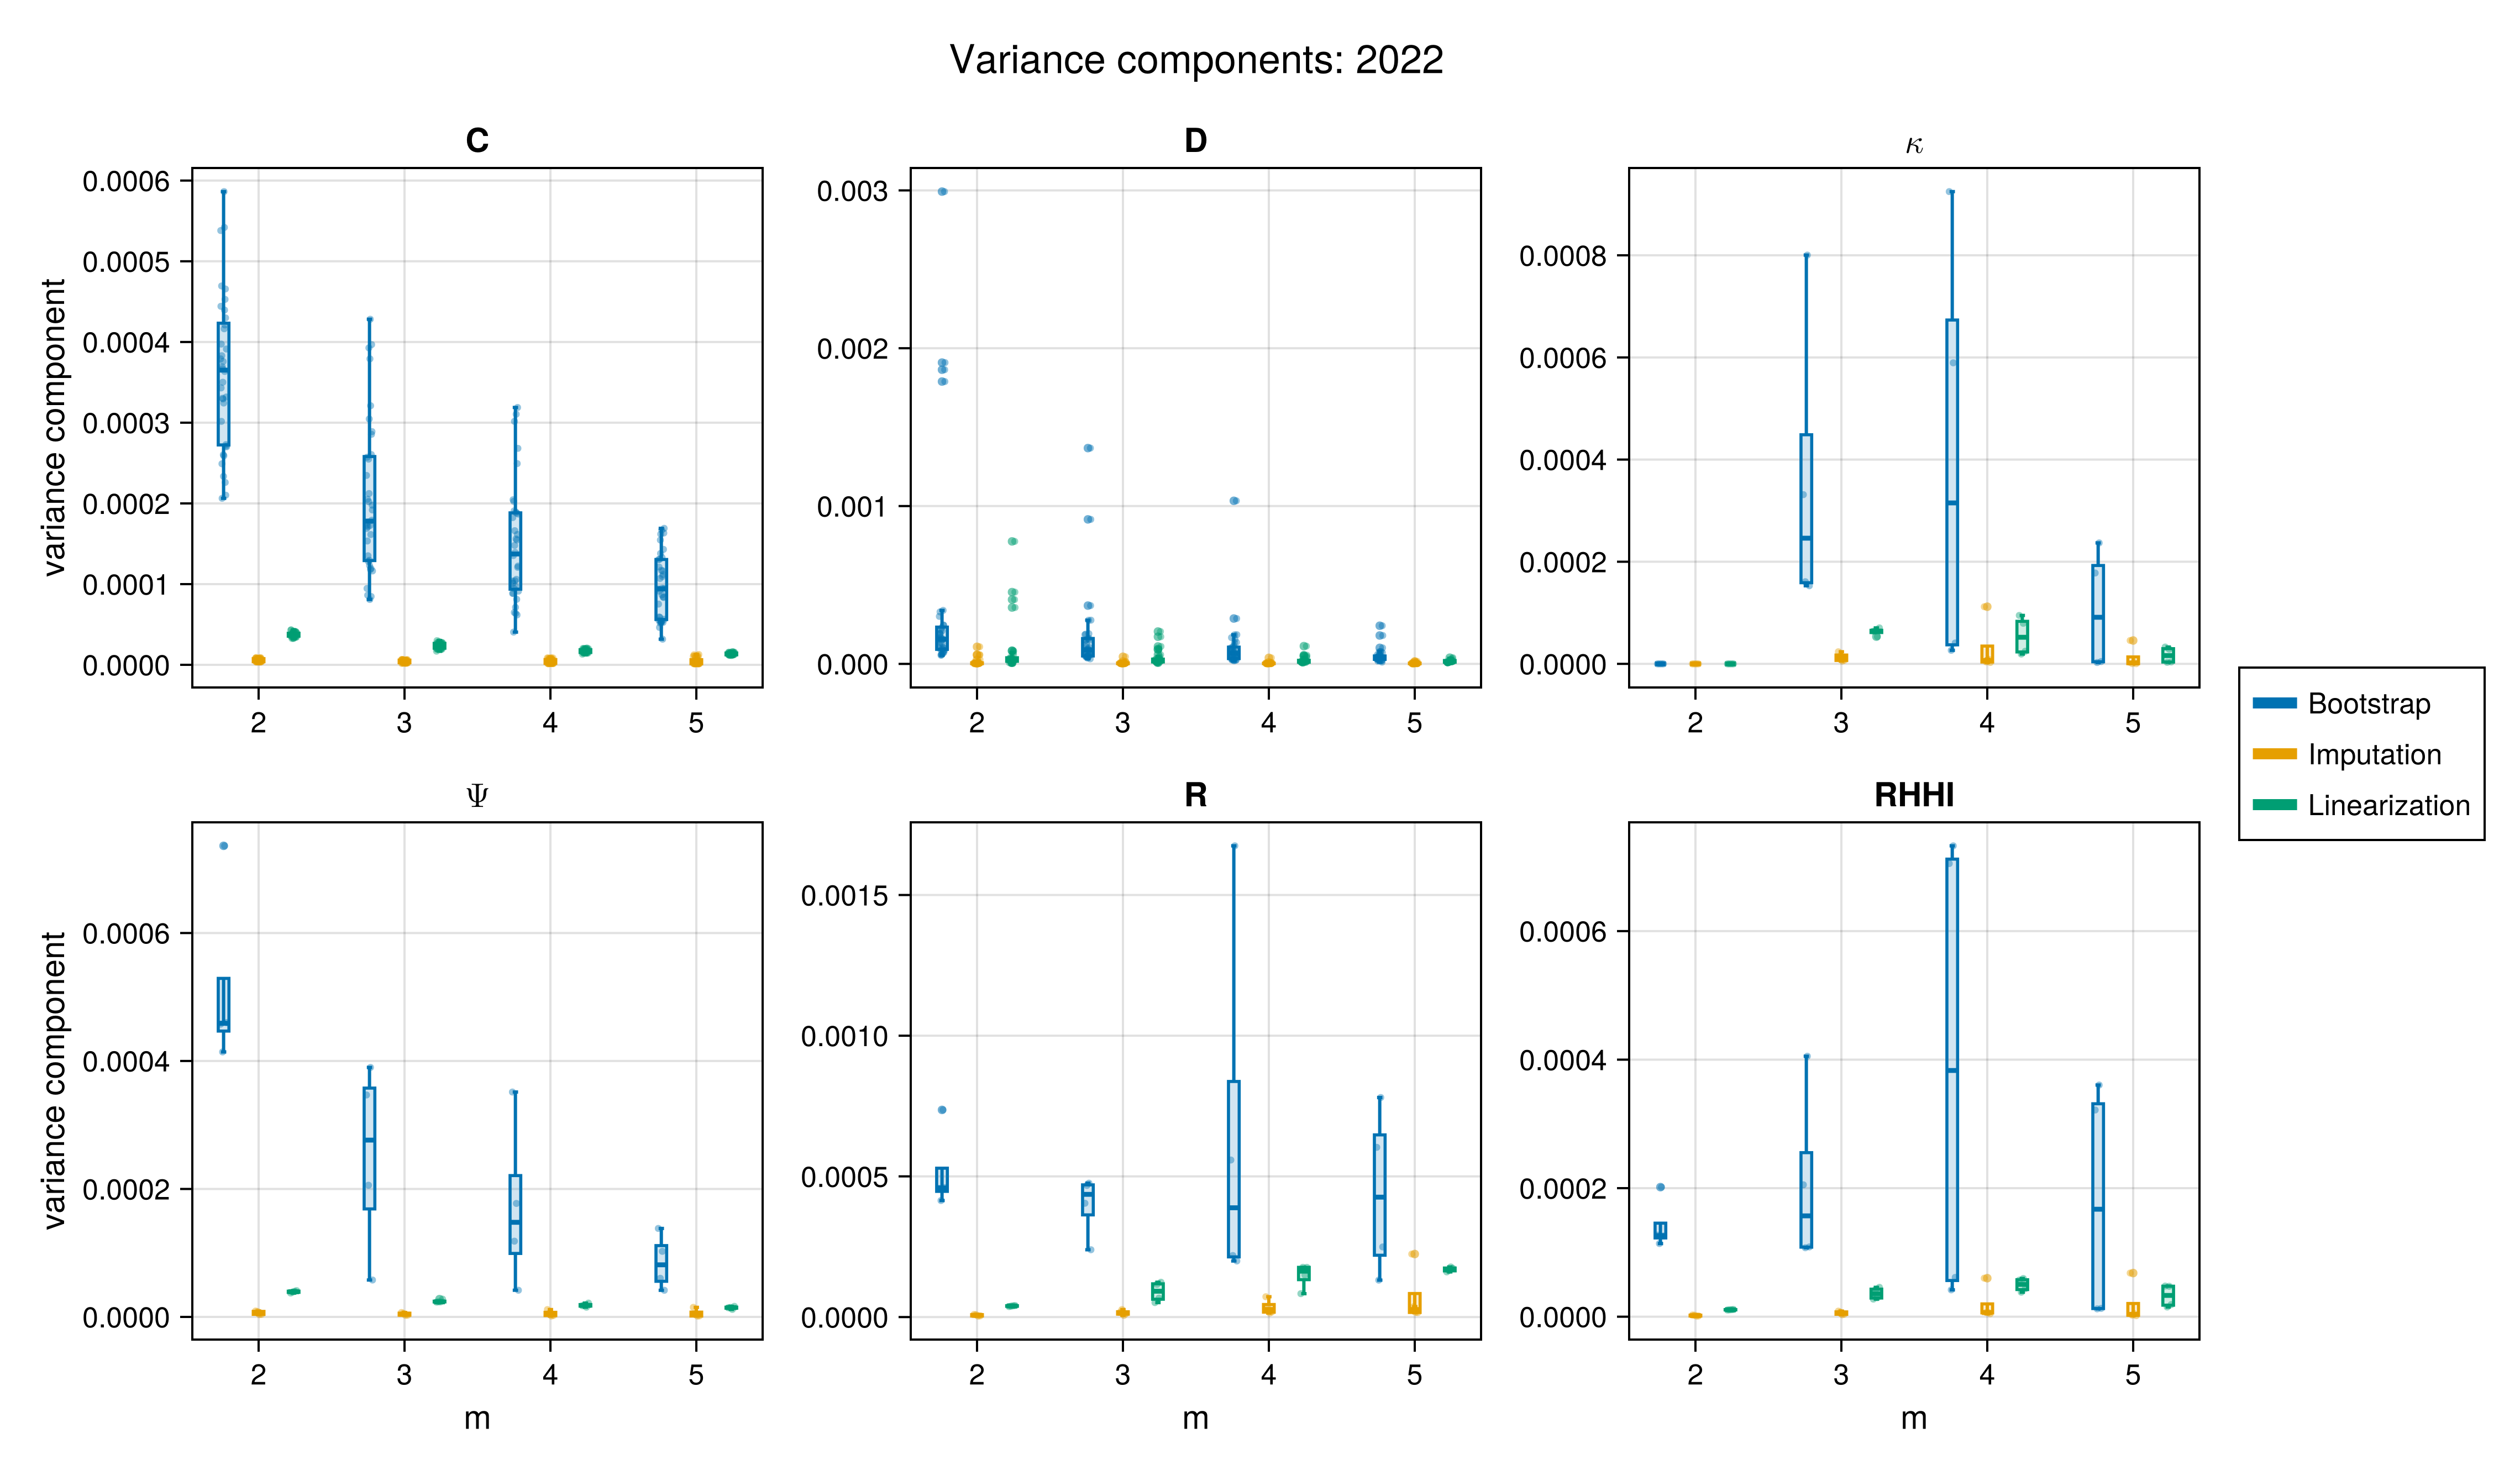
\includegraphics[width=\textwidth,height=\textheight,keepaspectratio]{imgs/variance_decomposition_2022.png}
\caption{Nested variance decomposition by measure and candidate-set size,
2022. The figure reports the bootstrap, imputation, and linearization variance
components for the measures used in the main analysis. For the group-based
measures, \(C\) and \(D\) pool the corresponding analysis cells across
available groupings.}
\label{fig:variance-decomposition-2022}
\end{figure}


The decomposition is descriptive. It does not introduce an additional
population model for the measures. Its purpose is to report how much of the
simulation variability in the measured profile, within a fixed analysis cell,
is attributable to weighted resampling, missing-data imputation, and stochastic
linearization.


A compact visualization of this decomposition is shown in Figure
\ref{fig:variance-decomposition-2022}. The figure reports, for the 2022 wave
and the selected scenario, the bootstrap, imputation, and linearization
variance components for the measures used in the main analysis. The horizontal
axis gives candidate-set size \(m\), and within each value of \(m\) the
boxplots compare the three nested variance components. For the group-based
measures, \(C\) and \(D\) pool the corresponding analysis cells across the
available groupings, so the figure should be read as a descriptive summary
across group diagnostics, not as a statement about one particular grouping
variable.

Several features stand out. First, the variance values are generally very
small in absolute magnitude. In most panels the components lie close to zero,
often in the range of small fractions of a percentage point. This is itself a
substantive result: although the pipeline contains several stochastic steps,
the resulting measures are typically quite stable within a fixed analysis cell.
The decomposition is therefore not uncovering large instabilities in the
measurement procedure, but rather a modest amount of simulation variability
whose relative composition can still be meaningfully compared across measures.

Second, most of the variance comes from the bootstrap stage. Across nearly all
measures and values of \(m\), the bootstrap component is visibly larger than
the imputation and linearization components. This means that most of the
simulation variability comes from changing the weighted pseudo-profile rather
than from the downstream stochastic operations applied to that pseudo-profile.
This pattern is especially clear for \(\Psi\), \(R\), \(\kappa\), and \(RHHI\),
but it also holds for the group-based measures \(C\) and \(D\).
In other words, once a bootstrap pseudo-profile is fixed, the additional
variability introduced by missing-data imputation and by stochastic
linearization is usually much smaller than the variability already induced by
resampling.

Third, the imputation and linearization components are typically small, although
their relative importance varies across measures. Linearization is usually more
visible than imputation in this run, especially for measures such as \(R\)
and \(RHHI\), while imputation remains comparatively modest across
most panels. Even so, both components remain well below the bootstrap
contribution in most cases.

Fourth, there is some heterogeneity across measures and across \(m\). Measures
such as \(D\) occasionally exhibit somewhat larger bootstrap
dispersion, and \(\kappa\) and \(RHHI\) show more uneven behavior as \(m\) changes.
This is unsurprising. Different measures respond differently to the geometry
and sparsity of the profile, and increasing \(m\) changes the ranking space
itself. Still, the broad qualitative pattern remains the same: candidate-set
size matters for the level of the components, but it does not overturn the
basic conclusion that the decomposition is dominated by bootstrap variability.

The corresponding figures for the other years are very similar. The exact
magnitudes differ across waves, scenarios, measures, and candidate-set sizes,
but the same basic structure reappears: leaf-level simulation variability is
generally small, most of it comes from bootstrap resampling, and the imputation
and linearization components are comparatively modest. The decomposition
therefore supports the view that the primary source of simulation variability
within fixed analysis cells is the sampling variation represented by the
weighted bootstrap, rather than instability introduced by the subsequent
handling of missing values or weak-order linearization.

\subsection{Candidate Set Selection}
For 2006, the availability criterion and substantive relevance coincide closely.
The five most available figures are Lula, Geraldo Alckmin, Heloísa Helena, José
Serra, and Cristóvam Buarque.\footnote{The weighted missingness order for 2006
is: Lula, 1.91\%; Geraldo Alckmin, 5.68\%; Heloísa Helena, 8.10\%; José Serra,
8.71\%; and Cristóvam Buarque, 19.18\%.} This set captures the incumbent
president, the main opposition candidate, a relevant left-wing dissident
candidacy, and nationally salient presidential or presidentially relevant
figures. I therefore use this order as the 2006 candidate sequence.

The 2018 case requires a different decision rule. If alternatives are selected
only by weighted missingness, the first names are Lula, Dilma Rousseff, Michel
Temer, Jair Bolsonaro, Fernando Haddad, Marina Silva, Aécio Neves, Ciro Gomes,
and Geraldo Alckmin.\footnote{The weighted missingness order for the leading
2018 figures is: Lula, 2.79\%; Dilma Rousseff, 4.15\%; Michel Temer, 5.95\%;
Jair Bolsonaro, 7.18\%; Fernando Haddad, 9.62\%; Marina Silva, 11.49\%; Aécio
Neves, 13.65\%; Ciro Gomes, 14.21\%; and Geraldo Alckmin, 14.68\%.} This
ordering is informative, but it is not an adequate rule for constructing the
2018 preference profile. It selects highly recognizable political figures,
including Lula, Dilma Rousseff, and Michel Temer, rather than only electorally
relevant presidential alternatives. Since Lula did not appear on the 2018
ballot, I do not include him as an alternative in the 2018 preference profile.
Instead, I use respondents' evaluation of Lula as a political-evaluative
partition in the group analysis. The 2018 candidate sequence is therefore
Fernando Haddad, Jair Bolsonaro, Ciro Gomes, Geraldo Alckmin, and Marina Silva.
This set captures the principal electoral alternatives in the presidential
contest while avoiding the conflation of notoriety with candidacy.

For 2022, the availability criterion again aligns more closely with electoral
relevance, with one important exception. The lowest-missingness figures are
Lula, Bolsonaro, Ciro Gomes, Marina Silva, Geraldo Alckmin, and Simone
Tebet.\footnote{The weighted missingness order for the leading 2022 figures is:
Lula, 1.43\%; Bolsonaro, 1.43\%; Ciro Gomes, 8.12\%; Marina Silva, 11.14\%;
Geraldo Alckmin, 11.30\%; and Simone Tebet, 18.29\%.} However, Geraldo Alckmin
was Lula's vice-presidential running mate in 2022 rather than an independent
presidential alternative. For this reason, I replace Alckmin with Simone Tebet,
who was an actual presidential candidate and occupied a substantively relevant
position in the electoral field. The 2022 candidate sequence is thus Lula,
Bolsonaro, Ciro Gomes, Simone Tebet, and Marina Silva.



\section{Supporting Results}
\subsection{Effective Rankings}

\begin{table}[!htbp]
\centering
\caption{Effective ranking and reversal-pair evolution}
\label{tab:effective-ranking-evolution}
\begin{tabular}{rrrrrrr}
\hline
m & EO 2006 & ENRP 2006 & EO 2018 & ENRP 2018 & EO 2022 & ENRP 2022 \\
\hline
2 & 1.77 & 1.00 & 1.87 & 1.00 & 1.98 & 1.00 \\
3 & 3.86 & 1.99 & 3.76 & 2.15 & 2.97 & 1.48 \\
4 & 11.14 & 5.67 & 9.62 & 4.18 & 6.60 & 3.02 \\
5 & 33.54 & 18.65 & 33.75 & 13.43 & 21.36 & 7.72 \\
\hline
\end{tabular}
\end{table}



\end{document}
